\section*{Learning Objectives}
\begin{itemize}
\item Mathematics is used to describe physical phenomena, pose engineering problems, and solve engineering problems. We close our Y1-introduction to Computational Linear Algebra by showing how linear algebra and computation allow you to use a notion of ``optimality'' as a criterion for selecting among a set of solutions to an engineering problem. 
\end{itemize}

\section*{Outcomes}
\begin{itemize}
\item Arg min should be thought of as another function in your toolbox,
$$x^\ast = \argmin_{x\in \real^m} f(x).$$
\item Extrema of a function occur at places where the function's first derivative vanishes.
\item The gradient of a function points in the direction of maximum rate of growth.
\item We will add to our knowledge of derivatives, specifically, second derivative.
\item Second-order optimization methods are based on root finding
\item Convex functions have global minima
\item Quadratic programs are special kinds of least squares problems
\item Optimization packages in Julia provide amazing tools for optimizing functions
\end{itemize}


\vspace*{1.5cm}





\newpage

\section{Motivation and Basic Ideas}

\begin{figure}[thb]%
\centering
\subfloat[]{%
    \label{fig:BowlScalarCost}%
	\centering
\includegraphics[width=0.45\columnwidth]{Chap12Optim/SimpleCost.png}}%
\hspace{5pt}%
\subfloat[]{%
    \label{fig:CurvyScalarCost}%
	\centering
\includegraphics[width=0.45\columnwidth]{Chap12Optim/LessSimpleCost.png}}%
\caption[]{(a) A ``simple'' cost function with a global minimum at $x^\ast=2$ and (b) a ``less simple'' cost function where there are two local minima, one at $x^\ast\approx 0.68$ and one at $x^\ast\approx 3.14$, as well as a local maximum at $\approx 2.1$.}
    \label{fig:ScalarCosts}
\end{figure}

Optimization is the process of finding one or more values $x\in \real^m$ that minimize a function $f: \real^m \to \real,$ 
where the scalar-valued function $f$ is called the \textbf{cost function}. The cost should be minimum at a point $x^\ast$ that is of interest to you, it should be ``small'' for values of $x$ that are ``near'' $x^\ast$ and it should be ``large'' for values of $x$ that are ``far'' from your preferred value, $x^\ast$. In Machine Learning, a cost function for minimization is also called a \textbf{regret function} in the sense that you regret being far from your preferred value, $x^\ast$, and your regret is minimum at $x^\ast$. We will abuse notation\footnote{Abusing notation means that one is being a bit sloppy with one's use of symbols, which is what notation is! One often abuses notation when doing the right thing is a bit painful and would cause more of a distraction to explain the good notation than to caution about using poor notation!} and write
\begin{equation}
    \label{eq:ArgMinAbuseNotation}
    x^\ast = \argmin_{x\in \real^m} f(x)
\end{equation}
to denote the value of $x$ achieving the minimum, even when there may be more than one such $x$.\\

One can also do the opposite of minimization, which is to \textbf{maximize a cost function}. In this case, the Machine Learning community calls the cost function a \textbf{reward}, because hey, who does not like to maximize reward and minimize regret! We will stick to minimization throughout the Chapter until the very end, when we'll discuss briefly how maximization and minimization are very closely related.\\

When $m=1$, that is, the cost function depends on a scalar variable, it is easy to graphically understand what minimization is all about. Figure~\ref{fig:BowlScalarCost} shows a ``bowl-shaped'' function that has a minimum at $x^\ast=2$. Moreover, if the function outside of the interval $[-1, 5]$ continues growing as shown, then $x^\ast=2$ is a \textbf{global minimum}, meaning that for all $x \neq x^\ast$, 
$$f(x^\ast) < f(x).$$ 
Even more special, if you imagine setting a marble on the curve at any point other than $x^\ast=2$, you can easily imagine the marble rolling and settling at the global minimum (assuming some friction).\\ 




On the other hand, Fig.~\ref{fig:CurvyScalarCost} presents a more complicated situation, where if the function outside of the interval $[-1, 5]$ continues growing as shown, then there is a global minimum at $x^\ast_a \approx 0.68$, but if you set a marble near $x=4$, you can imagine it getting stuck at the local bowl at $x^\ast_b \approx 3.14$, while if you start the marble at $x=1.5$, you can imagine it settling in at the local bowl  $x^\ast_a \approx 0.68$. The local bowls in the cost function are called \textbf{local minima} in that for all $x$ sufficiently near one of the $x^\ast_i$, 
$$f(x^\ast_i) \le f(x), $$
for $i\in \{a, b \}$.\\


\begin{figure}[htb]%
\centering
\subfloat[]{%
    \label{fig:BowlScalarCostDerivative}%
	\centering
\includegraphics[width=0.45\columnwidth]{Chap12Optim/SimpleCostDerivative.png}}%
\hspace{5pt}%
\subfloat[]{%
    \label{fig:CurvyScalarCostDerivative}%
	\centering
\includegraphics[width=0.45\columnwidth]{Chap12Optim/LessSimpleCostDerivative.png}}%
\caption[]{The derivatives of the cost functions have been added at strategic points. (a) A ``simple'' cost function with a global minimum at $x^\ast=2$ and (b) a ``less simple'' cost function where there are two local minima, one at $x^\ast\approx 0.68$ and one at $x^\ast\approx 3.14$, and a local maximum at $2.1$.}
    \label{fig:ScalarCostsDerivatives}
\end{figure}

\vspace*{.4cm}

\begin{tcolorbox}[sharp corners, colback=green!30, colframe=green!80!blue,title=\textbf{Derivative of the Cost Tells You How to Move Toward a Local Minimum}]
In Fig.~\ref{fig:ScalarCostsDerivatives}, we have plotted the derivatives of the cost functions at several points. Recall that the slope of the line segment at each point is equal to the derivative at that point. The plots tell us some really important things:
\begin{itemize}
    \item the derivative of the cost is zero at each local minimum;
    \item to the left of a local minimum, the derivative is negative (slope angles downward), while to the right of a local minimum, the derivative is positive (slope angles upward);
    \item hence, if you are at a point $x_k$, defining the next value as
\begin{equation}
    \label{eq:ScalarGradSearch}
    x_{k+1}=x_k - s \frac{d f(x_k)}{dx},
    \end{equation}
    where $s>0$ is called the \textbf{step size}, moves you in the direction of a local minimum (of course, if $s>0$ is too large, you can overshoot the local minimum); 
    \item because the derivative is zero at a local minimum, we can use the value of the derivative as a stopping criterion for the algorithm in \eqref{eq:ScalarGradSearch}; and
    \item the derivative also vanishes at local maxima, and hence if you start the algorithm in \eqref{eq:ScalarGradSearch} at a local maxima, you will be stuck there! 
\end{itemize}

\end{tcolorbox}



\begin{example}
\label{ex:ScalarCostMinimization}
Implement \eqref{eq:ScalarGradSearch} in Julia to find local minima of $f:\real\to \real$ by
$$f(x)=(x-2)^2 + 5 (\sin(x-2))^2 + 0.03(x+1)^3 + 4.$$

\end{example}

\textbf{Solution:} We wrote the Julia code given below and selected a set of initial conditions 
\begin{equation}
x_0 \in 
\left\{
\begin{array}{cccccccc}
-1.00 & 0.00 & 0.68 & 2.10 & 2.15 & 3.14 & 4.00 & 5.00 \\
\end{array}
\right\}
\end{equation}
for the Algorithm \eqref{eq:ScalarGradSearch} such that it would be started to the left and right of local minima and very close to the local maxima. The results are reported in \eqref{eq:resultsScalarGradSearch} for a step size of $h=0.1$ and in \eqref{eq:resultsScalarGradSearch02} for a step size of $h=0.2.$ The Algorithm converged quickly in all cases for a step size of $h=0.1$ and mostly failed for a step size of $h=0.2$ (we set a limit of $10^3$ iterations before terminating). \textbf{You have to chose your step sizes carefully!} for $h=0.1$, when started just to the left of the local maximum, the algorithm converged to the local minimum at $0.68$ and when started just to the right of the local maximum, it coverged to the local minimum at $3.14$.\\

\begin{lstlisting}[language=Julia,style=mystyle]
#Optimization
cost2(x)=(x.-2).^2 .+ 1 .- 5*(sin.(x.-2)).^2 .+ 3 .+ 0.03*(x.+1).^3
titre="Less Simple Example"
p2=plot(cost2,xmin,xmax,legend=false, title=titre, linewidth=3, color=:red )
s=0.2
delta=0.01
x0=[-1;0;0.68;2.1;2.15;3.14;4;5]
y0=cost2(x0)
IntermediateValues=Array{Float64}(undef, 0, 6)
for k =1:length(x0) #try various initial values of x0
    xk=x0[k]
   dcostdxk =( cost2(xk+delta)-cost2(xk-delta) )/(2*delta)
   fk=cost2(xk)
    j=0
    while (abs(dcostdxk)>1e-5)&(j < 1e3)
        j=j+1
        xk=xk-s*dcostdxk
        dcostdxk =( cost2(xk+delta)-cost2(xk-delta) )/(2*delta)
        fk=cost2(xk)
    end
    IntermediateValues=[IntermediateValues; j s x0[k] xk fk dcostdxk]
end
display(IntermediateValues)
# Show how to get latex code for printing matrices
using Latexify
set_default(fmt = "%.3f", convert_unicode = false)
latexify(IntermediateValues) |> print 
\end{lstlisting}


\begin{equation}
\label{eq:resultsScalarGradSearch}
\begin{array}{cccccc}
% \text{\bf N0.~Iterations}  &\hspace*{6mm} \mathbf{s} \hspace*{6mm} & \hspace*{9mm} \mathbf{x_0} \hspace*{9mm} &  \hspace*{7mm} \mathbf{x^\ast} \hspace*{7mm} & \hspace*{7mm} \mathbf{f(x^\ast)} \hspace*{7mm} & \hspace*{7mm} \mathbf{\frac{d f(x^\ast)}{dx}} \hspace*{7mm}\\
\text{\bf N0.~Iterations}  & \mathbf{s}  & \mathbf{x_0}  &  \mathbf{x^\ast} &  \mathbf{f(x^\ast)}  & \mathbf{\frac{d f(x^\ast)}{dx}} \\
\\
6 & 0.100 & -1.000 & 0.678 & 1.193 & 0.000 \\
6 & 0.100 & 0.000 & 0.678 & 1.193 & 0.000 \\
4 & 0.100 & 0.680 & 0.678 & 1.193 & 0.000 \\
\BLUE 15 & \BLUE 0.100 & \BLUE 2.100 & \BLUE 0.678 & \BLUE 1.193 & \BLUE 0.000 \\
\BLUE 12& \BLUE 0.100 & \BLUE 2.150 & \BLUE 3.137 & \BLUE 3.300 & \BLUE 0.000 \\
4 & 0.100 & 3.140 & 3.137 & 3.300 & 0.000 \\
7 & 0.100 & 4.000 & 3.137 & 3.300 & 0.000 \\
8 & 0.100 & 5.000 & 3.137 & 3.300 & 0.000 \\
\end{array}
\end{equation}

\vspace*{.3cm}

\begin{equation}
\label{eq:resultsScalarGradSearch02}
\begin{array}{rrrrrr}
\text{\bf N0.~Iterations} & \mathbf{s} \hspace*{3mm} & \mathbf{x_0} \hspace*{3mm}& \mathbf{x^\ast} \hspace*{3mm} & \mathbf{f(x^\ast)} \hspace*{1mm} & \mathbf{\frac{d f(x^\ast)}{dx}} \hspace*{1mm}\\
\\
\RED \text{FAILED~~~~} &  0.200 & -1.000 & \RED XX & \RED XX  & \RED XX  \\
\RED \text{FAILED~~~~} & 0.200 & 0.000 & \RED XX  & \RED XX  & \RED XX  \\
\RED \text{FAILED~~~~} & 0.200 & 0.680 & \RED XX   & \RED XX  & \RED XX  \\
\RED \text{FAILED~~~~} & 0.200 & 2.100 & \RED XX  & \RED XX  & \RED XX  \\
65 \hspace*{8mm}&  0.200 & 2.150 & 3.137 & 3.300 & 0.000 \\
47  \hspace*{8mm}& 0.200 & 3.140 & 3.137 & 3.300 & -0.000 \\
\RED \text{FAILED~~~~} & 0.200 & 4.000 & \RED XX   & \RED XX 1 & \RED XX  \\
69 \hspace*{8mm} & 0.200 & 5.000 & 3.137 & 3.300 & -0.000 \\
\end{array}
\end{equation}

\Qed.

\vspace*{.5cm}
We give next a more analytical take on our update law in \eqref{eq:ScalarGradSearch}. Which derivation is better? The intuition from plots or an analysis via linear approximations? The answer depends on how your brain is wired. I would say the best derivation is the one that gives you that ``ah ha'' moment!
\vspace*{.5cm}

\begin{tcolorbox}[title=\textbf{Linear Approximation to the Rescue!}]

Let's recall our linear approximation to a function $f : \real \to \real$ near a point $x_k$ by
\begin{equation}
    \label{eq:LinApproxRedux}
    f(x) \approx f(x_k) + \frac{df(x_k)}{dx} \left(x-x_k  \right).
\end{equation}
We seek to define $x_{k+1}$ so that $f(x_{k+1}) < f(x_k)$, that is, $f(x_{k+1}) - f(x_k) < 0$. We define $\Delta x_k := x_{k+1}-x_k$ and note that
\eqref{eq:LinApproxRedux} gives
\begin{equation}
    \label{eq:LinApproxRedux02}
    f(x_{k+1}) - f(x_k) \approx \frac{df(x_k)}{dx} \Delta x_k.
\end{equation} 
If we believe in the approximation (which is fine as long as $x_{k+1}$ is ``near'' $x_k$), then we can replace the approximation sign with an equals sign so that
\begin{equation}
    \label{eq:LinApproxRedux03}
    f(x_{k+1}) - f(x_k) < 0 \iff  \frac{df(x_k)}{dx} \Delta x_k < 0.
\end{equation} 
We see that if $ \frac{df(x_k)}{dx} =0$,  there is no choice of  $\Delta x_k$ that yields $  \frac{df(x_k)}{dx} \Delta x_k < 0$, which is why the derivative vanishing is our stopping criterion for a local extremum. We assume  therefore $ \frac{df(x_k)}{dx} \neq 0$, in which case
$$  \Delta x_k = - s\frac{df(x_k)}{dx} \implies \frac{df(x_k)}{dx} \Delta x_k = -s \left[  \frac{df(x_k)}{dx} \right]^2 < 0~~\text{for all}~~s>0, $$
and our update law becomes 
$$x_{k+1} = x_k + \Delta x_k =  x_k - s\frac{df(x_k)}{dx},$$
which agrees with \eqref{eq:ScalarGradSearch}. 
\end{tcolorbox}

%\vspace*{0.5cm}


%\newpage
\section{Contour Plots and the Gradient of the Cost}


\begin{figure}[thb]%
\centering
\subfloat[]{%
    \label{fig:NormSquaredSurface}%
	\centering
\includegraphics[width=0.45\columnwidth]{Chap12Optim/NormSquaredSurfacePlot.png}}%
\hspace{5pt}%
\subfloat[]{%
    \label{fig:NormSquaredcontour}%
	\centering
\includegraphics[width=0.45\columnwidth]{Chap12Optim/NormSquaredContourPlot.png}}%
\hspace{5pt}%
    \subfloat[]{%
    \label{fig:NormSquaredSurfaceAboutX0}%
	\centering
\includegraphics[width=0.45\columnwidth]{Chap12Optim/NormSquaredSurfacePlotAboutX0.png}}%
\hspace{5pt}%
\subfloat[]{%
    \label{fig:NormSquaredContourAboutX0}%
	\centering
\includegraphics[width=0.45\columnwidth]{Chap12Optim/NormSquaredContourPlotAboutX0.png}}%
    \caption[]{The graphs of two functions are shown in (a) and (c), with their corresponding contour plots shown in (b) and (d). Contour plots are lines where a function is constant. If you have ever used a topographical map when hiking, the lines on those maps indicate constant terrain height. In our case, the lines are constant $z=f(x_1,x_2)$ values as $(x_1,x_2)$ vary. Because the cost function we use here is very simple, its lines of constant contour are circles. More ``interesting'' examples will follow.}
    \label{fig:NormSquaredContourSurface}
\end{figure}

We acquired some good intuition by looking at plots of cost functions depending on a scalar variable $x\in \real$. We'll now augment our intuition by exploring the case $x\in \real^2$. We'll look at \textbf{contour plots of cost functions.} We'll also \textbf{encounter an important property of the gradient of a cost function that will generalize to arbitrary dimensions}.\\

We introduced the norm of a vector as a means to measure the length of vectors. We used the square of the norm in Chapter~\ref{sec:LeastSqauresGeneral} to find a \textit{least squared error solution} to a system of linear equations\footnote{Recall that used the square of the norm when assessing the error $e:=Ax-b$ in equations that do not have exact solutions.}. In engineering, the square of the norm is a very common cost function. In Fig.~\ref{fig:NormSquaredSurface} we plot 
$$f(x):=||x||^2=(x_1)^2 + (x_2)^2$$
on the $z$-axis versus $x_1$ and $x_2$. It's hard to imagine anything simpler to optimize! From the plot, we see a ``generalized bowl shape'', though it's hard to clearly identify where the minimum value occurs (yes, we know it occurs at $x=0$). To the right of the plot, in Fig.~\ref{fig:NormSquaredcontour}, we show a \textbf{contour plot} of $f(x_1,x_2)$. The circles about the origin show values of $x=(x_1,x_2)$ where the cost function is constant; in the inner circle, $f(x)=||x||^2=1$, then $f(x)=||x||^2=4$, $\ldots$, until $f(x)=||x||^2=25$. In the contour plot, it is easy to see where the minimum value occurs. \\

Similarly, in Fig.~\ref{fig:NormSquaredSurfaceAboutX0}, we show a plot of 
\begin{equation}
    \label{eq:offsetCircles}
    f(x)=||x-x_0||^2=(x_1-x_{01})^2 + (x_2-x_{02})^2
\end{equation}
for $x_0=[1; 2]$. In the corresponding contour plot, Fig.~\ref{fig:NormSquaredContourAboutX0}, it is equally easy to see where the minimum occurs. We will use the contour plots to show the correct direction to follow from a given point $x_k$ so that one moves efficiently toward a value of $x^\ast$ that is a local minimum.\\


Recall that the gradient of \eqref{eq:offsetCircles} is a row
\footnote{From Calculus, in this case, the exact formula is $\nabla f(x) = \left[~ 2(x_1-x_{01}) ~~~  2(x_2-x_{02})~\right]$} vector of the form $\nabla f(x)= \left[ \frac{\partial f(x)}{\partial x_1} ~~~ \frac{\partial f(x)}{\partial x_2}\right]$. Hence, the transpose of the gradient is a column vector in $\real^2$, namely
\begin{equation}
    \label{eq:GradientOffsetCircles}
    \left[ \nabla f(x) \right]^\top = \left[ \begin{array}{c} \frac{\partial f(x)}{\partial x_1} \\ \frac{\partial f(x)}{\partial x_2} \end{array} \right].
\end{equation}

Figure~\ref{fig:NormSquaredContourPlotAboutX0WithGradient} shows two contour plots. In addition, we have plotted in green arrows the gradients of the cost functions at several points and overlaid them on the contour plots. In both cases, the gradients are pointing in the direction of maximum increase of the function. It follows that the negative of the gradient is the direction of maximum decrease.


\begin{figure}[htb]%
\centering
\subfloat[]{%
    \label{fig:NormSquaredContourPlotAboutX0WithGradient}%
\centering
\includegraphics[width=0.45\textwidth]{Chap12Optim/NormSquaredContourPlotAboutX0WithGradient.png}
}
\hspace{5pt}%
\subfloat[]{%
    \label{fig:LeastSquaresContourPlotAboutX0WithGradient}%
	\centering
\includegraphics[width=0.45\columnwidth]{Chap12Optim/LeastSquaresContourPlotAboutX0WithGradient.png}}%
\caption[]{Contour Plots plus Gradients. (a) shows a very simple cost function, $||x-[1;2]||^2$, where the contours of constant cost are circles. (b) shows a more typical situation, where the contours are squeezed in one direction. In both cases, the gradients, plotted in green arrows, are pointing in the direction of maximum increase of the function. Hence, the negative of the gradient is the direction of maximum decrease. }
    \label{fig:ContourPlotsDerivatives}
\end{figure}

In Fig.~\ref{fig:ContourPlotsDerivatives}, we could not plot the gradients at the minima because the length of the gradient vector is zero at a (local) minimum! In case you want to see why this is true, from Calculus, one obtains that
    \begin{align}
        \label{eq:GradientVanishesAtMinimaScalarCase}
    \nabla \left((x_1-x_{01})^2 + (x_2-x_{02})^2 \right) &= 2 (x_1-x_{01}) + 2(x_2-x_{02}) \\
        \label{eq:GradientVanishesAtMinimaVectorExample}
    \nabla \left( (Ax-b)^\top \cdot (Ax-b) \right) & = 2 (Ax-b)^\top\cdot A.
    \end{align}
The minimum of $(x_1-x_{01})^2 + (x_2-x_{02})^2$ occurs at $x_1^\ast=x_{01}$ and $x_2^\ast=x_{02}$, and indeed, the gradient vanishes at $x^\ast$. The minimum of $||Ax-b||^2 = (Ax-b)^\top \cdot (Ax-b)$ satisfies $A^\top \cdot A x^\ast = A^\top b$, and direct substitution into the corresponding gradient shows that it vanishes as well. While this is not a proof, it gives you a hint that the gradient vanishing at a local minimum may be true.


\section{Gradient Descent}
\label{sec:GradientDescent}



\begin{tcolorbox}[sharp corners, colback=green!30, colframe=green!80!blue,title=\textbf{Gradient Descent}]

Equations \eqref{eq:GradientVanishesAtMinimaScalarCase} and \eqref{eq:GradientVanishesAtMinimaVectorExample} along with Fig.~\ref{fig:ContourPlotsDerivatives} tell us some really important things:
\begin{itemize}
\item the gradient vanishes at local minima;
    \item the gradient points in the direction of fastest growth of the cost function, and the negative of the gradient points in the direction of fastest decrease;
    \item hence, if you are at a point $x_k$, defining the next value as
\begin{equation}
    \label{eq:VectorGradientDescent}
    x_{k+1}=x_k - s \left[ \nabla f(x_k) \right]^\top,
    \end{equation}
    where $s>0$ is called the \textbf{step size}, moves you in the direction of a local minimum (of course, if $s>0$ is too large, you can overshoot the local minimum); 
    \item because the gradient is zero at a local minimum, we can use the value of the norm of the gradient as a stopping criterion for the algorithm in \eqref{eq:VectorGradientDescent}; and
    \item the gradient also vanishes at local maxima, and hence if you start the algorithm in \eqref{eq:VectorGradientDescent} at a local maxima, you will be stuck there.
\end{itemize}

\end{tcolorbox}

Before doing examples, we'll also show we can derive \eqref{eq:VectorGradientDescent} from the linear approximation of $f:\real^m \to \real$ near a point $x_k$, namely,
\begin{equation}
    \label{eq:LinApproxReduxGrad}
    f(x) \approx f(x_k) + \nabla f(x_k) \left(x-x_k  \right),
\end{equation}
where $\nabla f(x_k)$ is the gradient of $f$ at $x_k$ and is a $1 \times m $ row vector. 
We seek to define $x_{k+1}$ so that $f(x_{k+1}) < f(x_k)$, that is, $f(x_{k+1}) - f(x_k) < 0$. We define $\Delta x_k := x_{k+1}-x_k$ and note that
\eqref{eq:LinApproxReduxGrad} gives
\begin{equation}
    \label{eq:LinApproxReduxGrad02}
    f(x_{k+1}) - f(x_k) \approx \nabla f(x_k) \Delta x_k.
\end{equation} 
If we believe in the approximation (which is fine as long as $x_{k+1}$ is ``near'' $x_k$), then we can replace the approximation sign with an equals sign so that
\begin{equation}
    \label{eq:LinApproxReduxGrad03}
    f(x_{k+1}) - f(x_k) < 0 \iff  \nabla f(x_k)\Delta x_k < 0.
\end{equation} 
We see that if $ \nabla f(x_k) =0$, there is no choice of  $\Delta x_k$ that yields $  \nabla f(x_k)\Delta x_k 0 < 0$, which is why the gradient vanishing is our stopping criterion for a local extremum. We assume  therefore $ \nabla f(x_k) \neq 0$, in which case selecting
$$  \Delta x_k = - s\left[\nabla f(x_k)\right]^\top \implies \nabla f(x_k)\Delta x_k = -s ||\left[\nabla f(x_k)  \right]^\top||^2 < 0~~\text{for all}~~s>0. $$
Our update law is then 
$$x_{k+1} = x_k + \Delta x_k =  x_k - s\left[\nabla f(x_k)\right]^\top,$$
which agrees with \eqref{eq:VectorGradientDescent}. \\

\textbf{Remark:} There are easy variations of the Gradient Descent Algorithm,  \href{https://hal.archives-ouvertes.fr/hal-02096241/document}{Plestan-2020}. Let's note that our key condition is   $$ \nabla f(x_k)\Delta x_k < 0.$$
If we define the $i$-th component of $\Delta x_k$ by
$$ \left( \Delta x_k \right)_i:= \begin{cases} ~~~~~~0  & \frac{\partial f(x_k)}{\partial x_i}  = 0 \\
-s~~ {\rm sign}\left( \frac{\partial f(x_k)}{\partial x_i} \right) & \text{otherwise}\end{cases}, $$
then it is still true that $\nabla f(x_k)\Delta x_k < 0 \iff \nabla f(x_k) \neq 0_{1 \times m}$, and thus
we are moving in a descent direction. 

\begin{example}
\label{ex:VectorGradientDescent}
We'll re-visit the least squares problem from Chapter~\ref{sec:LinearRegression}, and use gradient descent as given in \eqref{eq:VectorGradientDescent} to solve $$x^\ast = \argmin_{x \in \real^m} ||Ax-b ||^2$$
and compare it to the closed-form solution
$ \left(A^\top A \right) x^\ast = A^\top b,$ for 
$$
A=\left[
\begin{array}{ccc}
1.0000 & 0.0000 & 0.0000 \\
1.0000 & 0.2500 & 0.0625 \\
1.0000 & 0.5000 & 0.2500 \\
1.0000 & 0.7500 & 0.5625 \\
1.0000 & 1.0000 & 1.0000 \\
1.0000 & 1.2500 & 1.5625 \\
1.0000 & 1.5000 & 2.2500 \\
1.0000 & 1.7500 & 3.0625 \\
1.0000 & 2.0000 & 4.0000 \\
\end{array}
\right]
~~~\text{and}~~~
b=
\left[
\begin{array}{c}
1.0000 \\
1.0000 \\
1.5000 \\
2.0000 \\
3.0000 \\
4.2500 \\
5.5000 \\
7.0000 \\
10.0000 \\
\end{array}
\right].
$$

\end{example}

\textbf{Solution:} We apply gradient descent as given in \eqref{eq:VectorGradientDescent} to the optimization problem, 
$$x^\ast = \argmin_{x \in \real^3}  \left(A x -b \right)^\top \left(  Ax-b \right).$$ 
We use symmetric differences to compute the gradient of
$$f(x):= \left(A x -b \right)^\top \left(  Ax-b \right), $$ set the step size to $s=0.01$, and the tolerance to $|| \nabla f(x_k) || < 10^{-5}$. After 2,673 iterations, we obtain
\begin{equation}
x^{\rm approx} = \left[
\begin{array}{r}
1.065144e+00 \\
-6.257368e-01 \\
2.454536e+00 \\
\end{array}
\right].
\
\end{equation}
For comparison purposes, we recall that the true answer is
\begin{equation}
x^\ast=\left[
\begin{array}{r}
1.065152e+00 \\
-6.257576e-01 \\
2.454545e+00 \\
\end{array}
\right].
\end{equation}

\Qed

%\newpage

The true power of optimization becomes clear when we use it to solve problems that do NOT have closed-form solutions. Check out the next section! \\



%%%%%%%%%%%%%%%%%%%%%%%%%%%%%%%%%%%%%%%%%%%%%%%%%%%%%%%%%
% BRUCE ADDED BELOW
%%%%%%%%%%%%%%%%%%%%%%%%%%%%%%%%%%%%%%%%%%%%%%%%%%%%%%%%%
% \jwg{\Huge Place an extrinsic calibration problem here? }
\section{Extrinsic Calibration Using Gradient Descent}
\label{sec:ExtrinsicCalibration}
Extrinsic calibration is the problem of finding a rotation matrix and a translation vector that allows one to transform the 3D-$(x,y,z)$ points measured by a LiDAR so as to align them with the data captured by a camera. The problem is interesting because it is easy to show visually what one wants to accomplish, but yet, how to formulate the objective mathematically is not clear at first glance, and for sure, there is no obvious ``equation'' to solve in order to compute a solution. 

Here, we'll go into enough detail that we can formulate an optimization problem for ``aligning'' the scenes observed by the LiDAR and the camera. We'll first address the optimization problem using gradient descent and later, we'll use a more efficient technique that uses ``higher-order'' information about the cost function. The difference in the rates of convergence is mind blowing.

\subsection{Introduction}
\label{ex:ExtrinsicCalibrationUsingGradientDescent}
 Currently, basic cameras provide many more data points (pixels) for a given surface size at a given distance than even high-end LiDARs. However, cameras rely on the consistency of the ambient lighting and provide less accurate depth estimation. On the other hand, LiDARs give accurate distance measurement, and rapidly changing ambient lighting will not affect measurements of a LiDAR. Due to these different inherent properties of LiDARs and cameras, it is necessary to ``fuse'' the LiDAR and the camera on Cassie's torso, as shown in Fig.~\ref{fig:CassieTorso}. By fusing, we mean overlaying a point cloud from a LiDAR to an image from a camera. The process of fusing two or more different types of data from different sensors is called an ``extrinsic calibration''. The problem requires high accuracy and precision; a little error in the process leads to an unusable result, as shown in Fig.~\ref{fig:MisCalibratedResult}.


\begin{figure}[htb]%
    \centering
    \subfloat[]{%
        \label{fig:CalibratedResult}%
         \includegraphics[trim=1100 40 0 100,clip,height=0.32\textwidth]{graphics/Chap12Optim/CalibrationRestuls.png}}%
        \hspace{5pt}
    \subfloat[]{%
        \label{fig:MisCalibratedResult}%
        \includegraphics[trim=10 10 1100 100,clip,height=0.32\textwidth]{graphics/Chap12Optim/CalibrationRestuls.png}}
    \caption[]{\subref{fig:CalibratedResult} shows good alignment of a LiDAR
            point cloud projected onto a camera image.
        \subref{fig:MisCalibratedResult} shows that a calibration result is not
        usable if it has a few degrees of rotation error and a few percent of
        translation error.
    }%
\label{fig:Calibration}%
\end{figure}
\begin{figure}[htb]%
    \centering
    \subfloat[]{%
        \label{fig:NormalTarget}%
        % l, b, r,t
        \includegraphics[trim=0 0 0 100,clip,height=0.3\textwidth]{graphics/Chap12Optim/target.png}}%
        \hspace{8pt}
        \subfloat[]{%
        \label{fig:EdgeDetectedlTarget}%
        % l b r t
    \includegraphics[trim=0 40 0 100,clip,height=0.3\textwidth]{graphics/Chap12Optim/EdgeDetectionTarget.png}}%
    \caption[]{\subref{fig:NormalTarget} shows a normal image and
    \subref{fig:EdgeDetectedlTarget} illustrates the result of edge detection applied
on \subref{fig:NormalTarget}.}% 
    \label{fig:EdgeDetection}%
\end{figure}



When we calibrate sensors, we need to find corresponding ``features'' captured from different sensors. Features are some specific structures in an environment, such as points, edges or corners, etc. Figure~\ref{fig:EdgeDetection} considers edges as features and extracts them out from an image. Once we find ``enough'' corresponding features, we want to estimate a ``rigid-body transformation'' between each sensor that we want to calibrate. A rigid-body transformation $H$ consists of a rotation matrix $R$ and a translation vector $t$ and is defined as
\begin{equation}
    H := 
    \begin{bmatrix}
    R & t\\
    0 & 1
    \end{bmatrix}.
\end{equation}
% {\text{from_sensor1}}^{\text{to_sensor2}}
When calibrating two sensors, it is good practice to indicate how the transformation is defined, by specifying that is a transformation from which sensor to which other sensor! We will use the notation $R_{\text{~from sensor1}}^{\text{~to sensor2}}$ and $t_{\text{~from sensor1}}^{\text{~to sensor2}}$ 
to represent the rotation and translation from the sensor 1 to sensor 2. \\

In the following, we will illustrate how to perform an extrinsic calibration between a LiDAR and a camera. We will walk you through the calibration process and provide some insight on how we try to take advantage of their relative strengths and avoid their weaknesses. All the images and data are collected from the torso of Cassie Blue, as shown in Fig.~\ref{fig:CalibratedResult}.
\begin{figure}[hbt]%
    \centering
    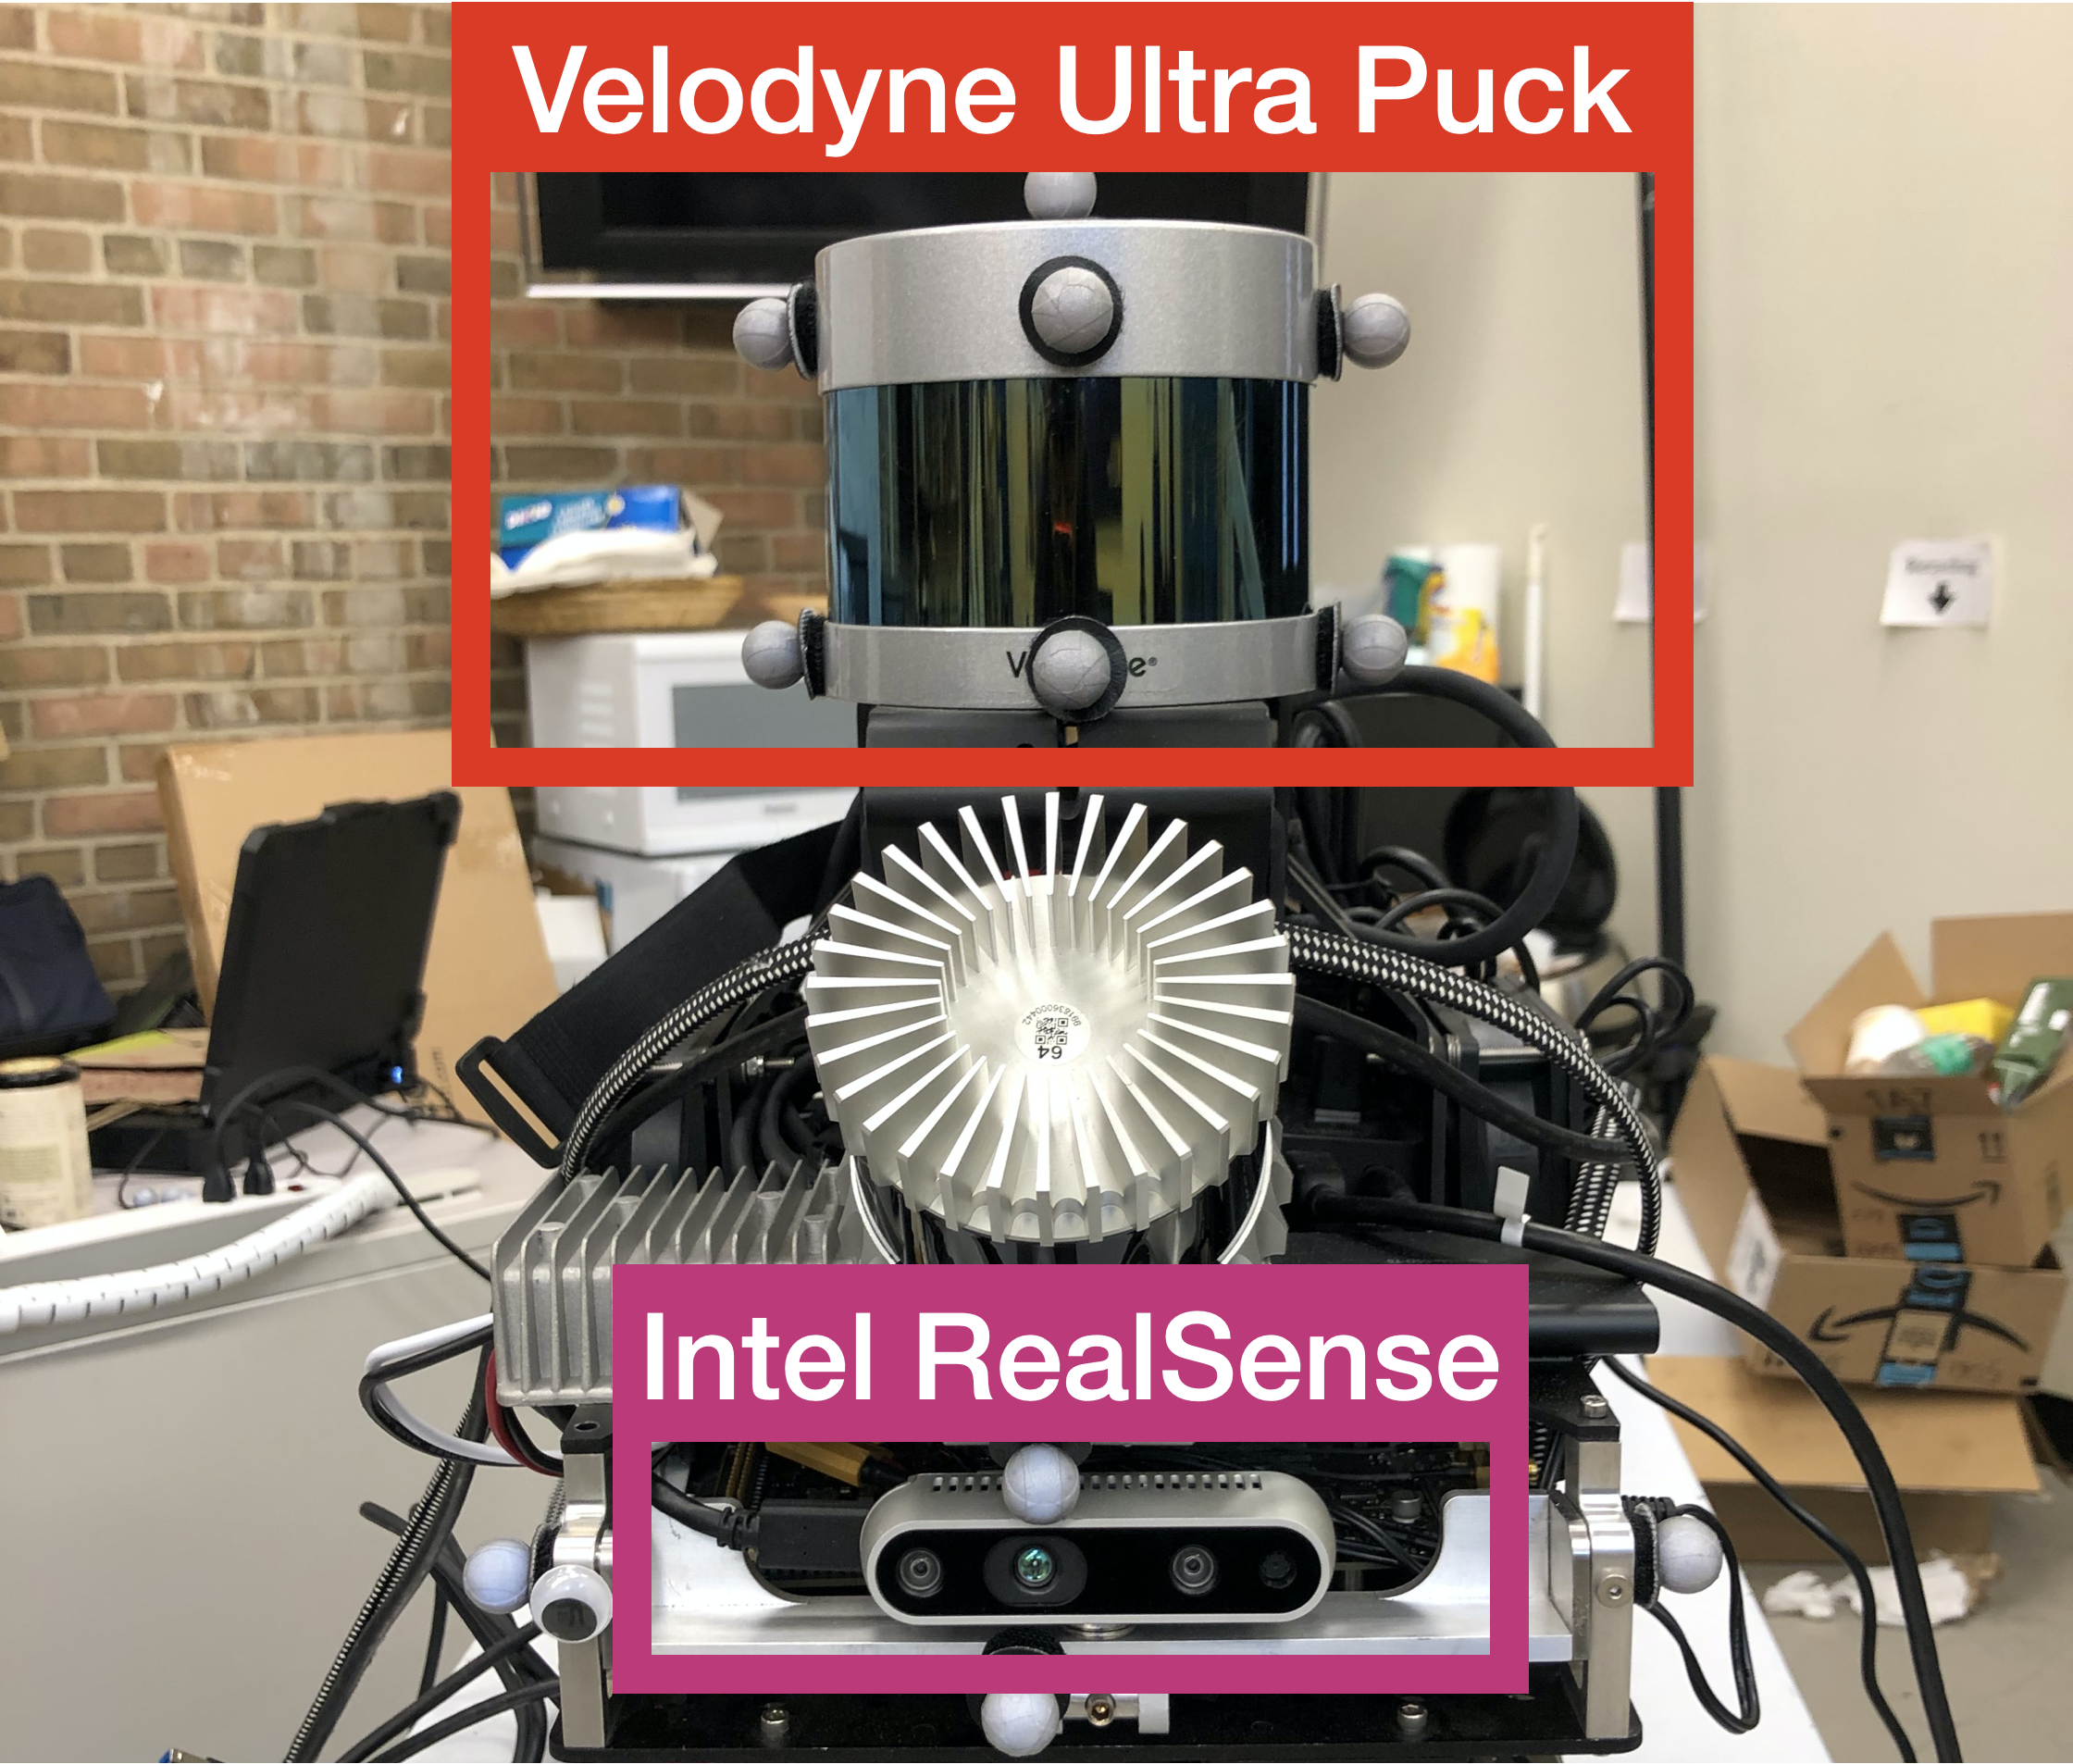
\includegraphics[trim=0 0 0 0,clip,height=0.36\textwidth]{graphics/Chap12Optim/CassieTorso.png}
\caption[]{This figure shows the torso of Cassie Blue. We use it in practice to do our \href{https://youtu.be/uFyT8zCg1Kk}{autonomy adventures}!}
\label{fig:CassieTorso}%
\end{figure}



% \jwg{In project 1, we used lowercase t for the translation vector. Let's go with that. No, i am in an NSF panel. Zooming! All day tomorrow too. I can work a little from time to time. You are doing fine. The projection map can be added. see the Appendix. } \bh{Sure, I can talk now if you have time to talk for a little. Okay, I will edit it. I am adding the projection map to the appendix. Yep. I am doing it now. I have several meetings this morning. }




\subsection{Problem Setup and Initial Solution}
In this problem, we take corners as our features, as shown in
Fig.~\ref{fig:CalibartionTargets}. In particular, we want to align the LiDAR
vertices (green dots) with the camera corners (red dots) in Fig.~\ref{fig:MisAlignmentTargets}. Additionally, we assume all corresponding corners
from the two sensors are already given\footnote{To
understand how to obtain corresponding corners, we encourage the readers to read
``\href{https://ieeexplore.ieee.org/document/9145571}{Improvements to Target-Based 3D
LiDAR to Camera Calibration},'' by Jiunn-Kai Huang and Jessy W. Grizzle.}, and the
process of feature extraction is uploaded to our
\href{https://www.youtube.com/watch?v=R2iMQt8tDhM}{YouTube
Channel}! Let $X$ and $Y$ be the features from a LiDAR and a camera, respectively. When
overlaying the two sets of features, we want the their respective coordinates in the camera frame to be as close as
possible. Therefore, the problem can be formulated as 
\begin{equation}
\label{eq:PnP}
\begin{aligned}
    \left({R_L^C}^*, {t_L^C}^*\right) &:=  \argmin_{R,t}f(R,t,X,Y) \\&
    := \argmin_{R, t}\sum_{i=1}^{4n}\|\Pi\left(X_i; R, t\right)-{}_{C}Y_i\|_2^2,
\end{aligned}
\end{equation}
where $R_L^C$ and $t_L^C$ are the rotation and translation from the LiDAR frame to the camera frame, $f$ is the cost function, and $\Pi$ is a projection map, which we will not dive
into in here, but is provided in Appendix~\ref{sec:ProjectionMap}. For now, you can
consider it as a black box that takes points in 3D space and maps them to their corresponding points on the 2D image-plane of the camera. We apply the gradient descent algorithm to solve
\eqref{eq:PnP} and the update function is:
\begin{equation}
    \label{eq:Gradient}
    H_{k+1}  = H_k - s[\nabla f(H_k, X, Y)]^\mathsf{T}.
\end{equation}
After 5745 iterations with a step size of 1e-8, the cost drops from 49750 to
12.12, and the result is shown in Fig.~\ref{fig:GradientResult}. Later, we will
introduce a second-order method, the ``Hessian,'' to solve this problem and you
will be amazed when the Hessian-based algorithm converges in 14 iterations! Knowledge is power! \\

\textbf{Remark:} If you look into the implementation, you will find out that we do not represent the rotation matrix with nine elements even through it is a $3 \times 3$ matrix, 
\begin{equation}
    R = \begin{bmatrix}
    r_{11} & r_{12} & r_{13} \\
    r_{21} & r_{22} & r_{23} \\
    r_{31} & r_{32} & r_{33}
    \end{bmatrix}.
\end{equation}
Instead, we use a fact you would learn in an upper level math course or a mechanics course, which says that any rotation matrix can be represented as the ``matrix exponential'' of a $3 \times 3$ skew symmetric matrix of the form
$$\Omega:=\left[ \begin{array}{ccc}0 & -\omega_3 & \omega_2 \\ \omega_3 & 0 & -\omega_1 \\ -\omega_2 & \omega_1 & 0 \end{array} \right], $$
Hence, a rotation matrix depends on only three parameters, $\left(\omega_1, \omega_2, \omega_3 \right)$. 
(It's hard to learn too much Linear Algebra; there is always one more useful fact!). Knowledge is power. Keep digging, and you will keep having fun.
%\clearpage



\begin{figure}[bth]%
    \centering
    \subfloat[]{%
        \label{fig:LiDARVertices}%
         \includegraphics[trim=0 10 0 70,clip,width=0.8\textwidth]{graphics/Chap12Optim/LiDARVertices.png}}\\
    \subfloat[]{%
        \label{fig:MisAlignmentTargets}%
        \includegraphics[trim=10 10 20 100,clip,height=0.31\columnwidth]{graphics/Chap12Optim/MisAlignmentTargetCorner2.png}}%
        \hspace{5pt}
    \subfloat[]{%
        \label{fig:AlignedTargets}%
         \includegraphics[trim=20 10 20 100,clip,height=0.31\textwidth]{graphics/Chap12Optim/AlignedTargetCorner.png}}%
    \caption[]{
        \subref{fig:LiDARVertices} shows the LiDAR returns on the targets in black and
        estimated vertices in red. 
        \subref{fig:MisAlignmentTargets} illustrates the initial state of the
        optimization in \eqref{eq:PnP}. Our goal is to move the green dots onto the red
        dots, or you can also imagine moving the yellow box to the magenta box.
        \subref{fig:AlignedTargets} demonstrates the result of calibration: the 
        LiDAR vertices (green dots) are successfully projected onto a camera corners
    (red dots). 
}%
    \label{fig:CalibartionTargets}%
\end{figure}
\begin{figure}[H]%
    \centering
    \includegraphics[trim=0 0 0 30,clip,height=0.36\textwidth]{graphics/Chap12Optim/Result.png}
\caption[]{This figure demonstrates the calibration result of the gradient descent
algorithm. It looks pretty good; there is still some misalignment. The main drawback of the algorithm would that a very small step size if often required to make it work.}
\label{fig:GradientResult}%
\end{figure}


%%%%%%%%%%%%%%%%%%%%%%%%%%%%%%%%%%%%%%%%%%%%%%%%%%%%%%%%%
% BRUCE ENDED HERE
%%%%%%%%%%%%%%%%%%%%%%%%%%%%%%%%%%%%%%%%%%%%%%%%%%%%%%%%%
\newpage 

\section{Optimization as a Root Finding Problem: the Hessian}

Gradient descent is a powerful method to solve optimization problems and we've seen it in two contexts so far: finding a (local) minimum of a cost function that depends on a scalar variable $x$ in \eqref{eq:ScalarGradSearch}, and  finding a (local) minimum of a cost function that depends on a vector variable $x =\left(x_1, x_2, \ldots, x_m  \right)$ in \eqref{eq:VectorGradientDescent}. Our stopping criterion was $|\frac{df(x_k)}{dx}|$ ``sufficiently small'' for scalar problems and $||\left[\nabla f(x_k)\right]^\top||$ ``sufficiently small'' for vector problems. In other words, a (locally) optimal solution $x^\ast$ satisfies $\sfrac{df(x^\ast)}{dx}=0$ for scalar problems and $\nabla f(x^\ast)=0$ for vector problems. Said yet another way, our locally minimizing solutions are \textbf{roots of the derivative of the cost function}. \\


\begin{tcolorbox}[title =\textbf{\Large  Relation to Root Finding}]

Suppose we seek a point $x^\ast \in \real$ achieving a local minimum (or maximum) of a function $f: \real \to \real$. We know that a necessary condition is the derivative of $f$ vanishes at $x^\ast$, that is,
$$\left. \frac{df(x)}{dx} \right| _{x = x^\ast} = 0.$$
We note that the first derivative is just another real-valued function, namely, 
$$  \frac{df(x)}{dx}: \real \to \real.$$
Hence, we can say that for $x^\ast$ to achieve a minimum (or maximum) of the function $f:\real \to \real$, it must be a \textbf{root of} $ \frac{df(x)}{dx}: \real \to \real$. If we apply Newton's Method to the function $g(x): = \frac{df(x)}{dx}$ to find its roots, we'll need to find the first derivative of $g(x)$, which will lead us to the second derivative of the original function $f(x)$. This may sound overwhelming or intimidating, but shortly we will disabuse you of such concerns! \\

Next, suppose we seek a vector $x^\ast \in \real^m$ that achieves a local minimum (or maximum) of a function $f: \real^m \to \real$. We know that a necessary condition is the \textbf{gradient} of $f$ vanishes at $x^\ast$, that is,
$$ \nabla f(x^\ast) = 0_{1 \times m}.$$
We note that the \textbf{transpose of the gradient} is just another vector-valued function, namely, 
$$ {\nabla f(x)}^\top: \real^m \to \real^m;$$
we use the transpose to turn a row vector into a column vector. Because the gradient must vanish at a local min (or max), we can say that for $x^\ast$ to be a local minimum (or maximum) of the function $f:\real^m \to \real$, it must be a \textbf{root of} $ {\nabla f(x)}^\top: \real^m \to \real^m$. If we apply the Newton-Raphson Method to the function $g(x): = {\nabla f(x)}^\top$ to find its roots, we'll need to find the Jacobian of $g(x)$, which will lead us to a vector-version of the second derivative of the original function $f(x)$. This may sound overwhelming or intimidating, but shortly, we will once again disabuse you of such concerns! The Jacobian of the gradient has a cool name, \textbf{the Hessian}.
    
\end{tcolorbox}


In Chapter~\ref{chap:NonlinearEquations}, we learned a lot about finding roots of nonlinear equations. We will now apply that knowledge to optimization and thereby arrive at a more powerful optimization algorithm that uses information about the second derivative of the cost function! That sounds pretty wild and scary, but you'll see that it's very do-able. 

\subsection{Second Derivatives}
\label{sec:SecondDerivative}

Calculus has developed some good notation over the past 300 plus years and we will use it. The second derivative of a function  $f:\real \to \real $ is the first derivative of the function's first derivative, and is written like this,
\begin{equation}
    \label{eq:secondDerivative}
    \frac{d^2 f(x)}{dx^2}: = \frac{d}{dx}\frac{df(x)}{dx}.
\end{equation}
Let's write down the derivative of the derivative using the symmetric difference approximation to the derivative. We first recall that
\begin{equation}
\label{eq:symmetricDifferenceRecall}
   \frac{df(x)}{dx}\approx \frac{f(x + h)- f(x-  h)}{2 h},
\end{equation}
where $h>0$ is a small number. 
Let's use $\delta>0$ instead of $h$ for a small positive change in $x$ when writing down the second derivative as a symmetric difference
\begin{equation}
    \label{eq:secondDerivativeB}
    \begin{aligned}
    \frac{d^2 f(x)}{dx^2}&\approx\frac{ \frac{df(x+\delta)}{dx} -  \frac{df(x-\delta)}{dx} }{2 \delta}.
    \end{aligned}
\end{equation}
We now substitute \eqref{eq:symmetricDifferenceRecall} into \eqref{eq:secondDerivativeB} to obtain
\begin{equation}
    \label{eq:secondDerivativeC}
    \begin{aligned}
    \frac{d^2 f(x)}{dx^2}&\approx\frac{ \left[ \frac{f(x + \delta + h)- f(x + \delta -  h)}{2 h}  \right]-   \left[ \frac{f(x - \delta + h)- f(x - \delta -  h)}{2 h}  \right]}{2 \delta} \medskip\\
    & = \frac{ \left[f(x + \delta + h)- f(x + \delta -  h) \right]-   \left[ f(x - \delta + h)- f(x - \delta -  h) \right]}{4 h \delta} \medskip \\
     & = \frac{ f(x + \delta + h)- f(x + \delta -  h) -   f(x - \delta + h) +  f(x - \delta -  h) }{4 h \delta}.
    \end{aligned}
\end{equation}

Equation~\eqref{eq:secondDerivativeC} is a perfectly fine expression for the second derivative. At least for your author, keeping $\delta$ and $h$ separate made it easier to evaluate the individual terms and see how they appeared in the equation. Your experience may vary! It's more traditional to take $\delta = h$, which we now do so as to arrive at our final expression,
\begin{equation}
    \label{eq:secondDerivativeD} \boxed{
    \frac{d^2 f(x)}{dx^2}\approx \frac{ f(x + 2h)- 2 f(x )  +  f(x -2 h) }{4 h^2}
    }.
\end{equation}

In terms of coding, computing a numerical approximation to the second derivative is not much different than approximating the first derivative. Comparing \eqref{eq:secondDerivativeD} to \eqref{eq:symmetricDifference}, we see there is one more term to compute and instead of dividing by $2h$, we divide by $4 h^2$. \\

Note that if you took $h>0$ to be something relatively ``small'', such as $10^{-3}$, then $h^2$ is now really small, such as  $10^{-6}$. Be careful that you do not approach ``machine epsilon'' when doing your approximate derivatives!

\subsection{The Hessian is the Jacobian of the Transpose of the Gradient}
\label{sec:Hessian}

As the title of this section suggests, we define the \textbf{Hessian} of a function $f:\real^m \to \real$ as the Jacobian of the transpose of the gradient of the function. Using notation that comes to us from Calculus, we have that 
\begin{equation}
    \label{eq:Hessian}
    \nabla^2 f(x) := \frac{\partial}{\partial x} \left[ \nabla f(x) \right]^\top,
\end{equation}
where $ \nabla^2 f(x)$ is the notation for the Hessian of $f$ at the point $x$. We underline that here, the function $f$ depends on a vector $x \in \real^m$ and that $f(x) \in \real$ is a scalar. If $f(x) \in \real^n$, for $n > 1$, then the above formula makes no sense...it is just a bunch of meaningless symbols.\\

Equation \eqref{eq:Hessian} is a lot of notation packed into one tiny formula! Let's unpack it so as to understand it bit by bit. For a function $f: \real^m \to \real$, the transpose of its gradient is
\begin{equation}
\label{eq:OptimizatinGradient}
        \left[ \nabla f(x) \right]^\top :=  \left[\begin{array}{c}
      \frac{\partial f(x)}{\partial x_1} \\  \vdots \\ \frac{\partial f(x)}{\partial x_k} \\ \vdots \\ \frac{\partial f(x)}{\partial x_m}
    \end{array} \right].
\end{equation}
Moreover, we can approximate the indicated partial derivatives using symmetric differences,
\begin{equation}
    \label{eq:VectorPartialDerivative}
    \frac{\partial f(x)}{\partial x_k} = \frac{f(x+h e_k)-f(x-h e_k)}{2h},
    \end{equation}
where $\{e_1, \ldots,  e_k, \ldots, e_m \}$ is the natural basis vectors for $\real^m$.
For a function $g: \real^m \to \real^m$, we recall that its Jacobian is
\begin{equation}
    \label{eq:HessianB}
       \frac{\partial g(x)}{\partial x}:=  \left[\begin{array}{ccccc}
      \frac{\partial g(x)}{\partial x_1} &  \cdots & \frac{\partial g(x)}{\partial x_j} & \cdots & \frac{\partial g(x)}{\partial x_m}
    \end{array} \right].
\end{equation}
Moreover, we know how to numerically approximate the partial derivatives in \eqref{eq:HessianB} using symmetric differences and selecting $\delta >0$ by
\begin{equation}
    \label{eq:VectorPartialDerivative2}
    \frac{\partial g(x)}{\partial x_j} = \frac{g(x+\delta e_j)-g(x-\delta e_j)}{2 \delta}.
    \end{equation}\\
    
    
To put all of this together, we take
$$g(x):= \left[ \nabla f(x) \right]^\top $$
and apply \eqref{eq:VectorPartialDerivative2} to obtain a first numerical approximation for the Hessian, namely
\begin{equation}
    \label{eq:HessianNumerical} \small
    \nabla^2 f(x) \approx  
\frac{1}{2\delta} \left[\begin{array}{ccccc}
   \big(  \nabla f(x+\delta e_1)-\nabla f(x-\delta e_1)  \big)^\top 
   &  \cdots & \big( \nabla f(x+\delta e_k)-\nabla f(x-\delta e_k) \big)^\top
   & \cdots & \big( \nabla f(x+\delta e_m)-\nabla f(x-\delta e_m) \big)^\top
    \end{array} \right].
\end{equation}
Going one step further, if we let $\left[ \nabla^2 f(x)  \right]_{ij}$ be the $ij$-entry of the Hessian matrix (that is, the entry for its $i$-th row and $j$-th column), using \eqref{eq:VectorPartialDerivative}, we have that
\begin{equation}
    \label{eq:HessianNumericalB} \small
   \left[ \nabla^2 f(x)\right]_{ij} \approx  
\frac{1}{4 h \delta} 
   \big(   f(x+ h e_i + \delta e_j)-  f(x+ h e_i-\delta e_j) - f(x- h e_i + \delta e_j) +  f(x- h e_i-\delta e_j)\big) .
\end{equation}
In this case, setting $\delta=h$ does not really simplify the expression. In Julia, we suspect that you will find \eqref{eq:HessianNumerical} the easiest to implement. \\

\textbf{Remark:} In Calculus, we also use the notation
$$ \frac{\partial^2 f(x)}{\partial x_i \partial x_j} :=\left[ \nabla^2 f(x)\right]_{ij}.  $$
In \eqref{eq:HessianNumericalB}, when you take  $h = \delta$, you can see that $$\left[ \nabla^2 f(x)\right]_{ji} =\left[ \nabla^2 f(x)\right]_{ij}$$
and therefore the Hessian is a symmetric matrix. 

\subsection{Use of the Second Derivative and Hessian in Optimization}
\label{sec:HessianOptimization}

The most accessible forms of second-order optimization methods are based on applying Newton's method to the first derivative of a cost function that depends on a scalar variable $x\in \real$ or the Newton-Raphson Algorithm to the (transpose of the) gradient of a cost function that depends on a vector variable $x\in \real^m$. \\


\begin{tcolorbox}[sharp corners, colback=green!30, colframe=green!80!blue,title=\textbf{\Large Optimization as a Form of Root Finding: Scalar Decision Variable }]

For $f:\real \to \real$, the iterative process
\begin{equation}
    \label{eq:NewtonMethod02Optimization}
x_{k+1}=x_{k} - \left(   \frac{d^2f(x_k)}{dx^2}\right)^{-1} \frac{ df(x_k)}{dx}
\end{equation}
will converge to a local extremum of $f$ if the initial value $x_0$ is ``well chosen''. Because the algorithm is looking for \textbf{roots} of the first derivative, it is \textit{indifferent} to whether the root is a local minimum or a local maximum. \textbf{In Calculus, you will learn that if the second derivative is positive at a point where the first derivative vanishes, then you have found a local minimum.} Similarly, a negative second derivative implies a local maximum. \\

The damped version of the algorithm 
\begin{equation}
    \label{eq:NewtonMethodDampedOptimization}
x_{k+1}=x_{k} - s \left(   \frac{d^2f(x_k)}{dx^2}\right)^{-1} \frac{ df(x_k)}{dx},
\end{equation}
where $0< s < 1$, typically performs better in practice. We note that the second derivative, $\frac{d^2f(x)}{dx^2}$, can be approximated as in \eqref{eq:secondDerivativeD}.\\

\textbf{All of the remarks made in Chapter~\ref{chap:NonlinearEquations} about the validity of Newton's Algorithm apply here was well.}
\end{tcolorbox}

\begin{tcolorbox}[sharp corners, colback=green!30, colframe=green!80!blue,title=\textbf{ \Large Optimization as a Form of Root Finding: Vector Decision Variables}]
 For $f:\real^m \to \real$, the iterative process
\begin{align}
\label{eq:NewtonRaphsonOptimizationStep1}
\nabla^2 f(x_k)~ \Delta x_{k} &= - \left[\nabla f(x_k) \right]^\top \hspace*{0.3cm}(\text{solve for}~~\Delta x_k)  \\
\label{eq:NewtonRaphsonOptimizationStep2}
x_{k+1}&= x_k + \Delta x_{k}~~\hspace*{0.57cm}(\text{use~~} \Delta x_k ~~\text{to update our estimate of the optimal value})
\end{align}
will converge to a local extremum of $f$ if the initial value $x_0$ is ``well chosen''. Because the algorithm is looking for \textbf{roots} of the gradient, it is \textit{indifferent} to whether the root is a local minimum, a local maximum, or what is called a ``saddle point''. \textbf{In Calculus, you will learn that if the Hessian is positive definite at a point where the gradient vanishes, then you have found a local minimum.} Similarly, a negative definite Hessian implies a local maximum. A discussion of these nice properties is beyond the scope of ROB 101.\\


While for toy problems, we can use the matrix inverse to solve \eqref{eq:NewtonRaphsonOptimizationStep1} for $\Delta x_{k}$, for larger problems, we recommend using an LU Factorization or a QR Factorization. Once \eqref{eq:NewtonRaphsonOptimizationStep1}  has been solved, $x_{k+1}$ is updated in \eqref{eq:NewtonRaphsonOptimizationStep2} and the process repeats.
In practice, the \textbf{damped} version of the algorithm often works better, where one replaces \eqref{eq:NewtonRaphsonOptimizationStep2} with   
\begin{equation}
    \label{eq:NewtonRaphsonOptimizationStep3}
x_{k+1}= x_k + s \Delta x_{k},
\end{equation}
for some $0< s < 1$. We note that the Hessian, $\nabla^2f(x)$, can be approximated with either \eqref{eq:HessianNumerical} or \eqref{eq:HessianNumericalB}.\\

\textbf{All of the remarks made in Chapter~\ref{chap:NonlinearEquations} about the validity of the Newton-Raphson Algorithm apply here was well.}\\

\end{tcolorbox}

\begin{tcolorbox}[title = {\bf Don't be Intimidated by the Notation!}]

    While the equation $$\nabla^2 f(x_k)~ \Delta x_{k} = - \left[\nabla f(x_k) \right]^\top
$$ may look intimidating, it is just another linear equation $Ax = b$ where $A \leftrightarrow \nabla^2 f(x_k)$, a square matrix, $x \leftrightarrow \Delta x_{k}$, a column vector of unknowns,  and $b \leftrightarrow  - \left[\nabla f(x_k) \right]^\top$ is a column vector on the right-hand side of the equation. Hence, computing $\Delta x_{k}$ is cake for you by now.
\end{tcolorbox}



We re-do several of the previous examples.

\begin{example}
\label{ex:ScalarCostMinimizationReDo}
Based on Example~\ref{ex:ScalarCostMinimization},  but this time, we implement \eqref{eq:NewtonMethod02Optimization} and \eqref{eq:NewtonMethodDampedOptimization} in Julia to find local extrema of $f:\real\to \real$,
$$f(x)=(x-2)^2 + 5 (\sin(x-2))^2 + 0.03(x+1)^3 + 4.$$

\end{example}

\textbf{Solution:} We run the algorithm from the same initial conditions as in Example~\ref{ex:ScalarCostMinimization} and for two values of the step size, $s \in \{0.25, 1.0 \}$. The reader should note that we got somewhat lucky, and each time the algorithm converged to a root of the first derivative! We've highlighted in blue where the algorithm actually converged to a local maximum instead of a local minimum. How could we tell? The second derivative being positive implies a local minimum while it being negative implies a local maximum.\\

We note that the rate of convergence is much faster than for gradient descent (here, faster means fewer iterations of the algorithm). Finally, we note that the point to which the algorithm converges does depend on the initial condition. In fact, for $s=0.25$ and $s=1.0$, the algorithm sometimes converges to different roots of the first derivative, even when initialized at the same point.\\

If you can design a cost function so that it has a single extrema and it is your desired minimum, then you can avoid many of these problems. We talk a little about this in the section on ``Local vs Global''. 

\begin{equation}
\begin{array}{rrrrrrr}
\text{\bf N0.~Iterations} & \mathbf{s} \hspace*{7mm} & \mathbf{x_0} \hspace*{7mm}& \mathbf{x^\ast} \hspace*{7mm} & \mathbf{f(x^\ast)} \hspace*{7mm} & \mathbf{\frac{d f(x^\ast)}{dx}} \hspace*{7mm}
& \mathbf{\frac{d^2 f(x^\ast)}{dx^2}} \hspace*{7mm}\\
\\
2.2000e+01 & 1.0000e+00 & -1.0000e+00 & 3.1369e+00 & 3.3002e+00 & -4.5648e-09 & 9.2092e+00 \\
4.0000e+00 & 1.0000e+00 & 0.0000e+00 & 6.7838e-01 & 1.1926e+00 & -5.9785e-07 & 1.1085e+01 \\
2.0000e+00 & 1.0000e+00 & 6.8000e-01 & 6.7838e-01 & 1.1926e+00 & 6.9886e-10 & 1.1085e+01 \\
\BLUE \bf 2.0000e+00 & \BLUE \bf 1.0000e+00 & \BLUE \bf 2.1000e+00 & \BLUE \bf 2.1099e+00 & \BLUE \bf 4.8543e+00 & \BLUE \bf -1.6541e-08 & \BLUE \bf -7.1982e+00 \\
\BLUE \bf 2.0000e+00 & \BLUE \bf 1.0000e+00 & \BLUE \bf 2.1500e+00 & \BLUE \bf 2.1099e+00 & \BLUE \bf 4.8543e+00 & \BLUE \bf 5.2104e-07 & \BLUE \bf -7.1982e+00 \\
2.0000e+00 & 1.0000e+00 & 3.1400e+00 & 3.1369e+00 & 3.3002e+00 & -2.8692e-09 & 9.2092e+00 \\
5.0000e+00 & 1.0000e+00 & 4.0000e+00 & 3.1369e+00 & 3.3002e+00 & -2.6010e-09 & 9.2092e+00 \\
2.3000e+01 & 1.0000e+00 & 5.0000e+00 & -2.4271e+01 & 3.1198e+02 & 1.2562e-09 & 4.3032e+00 \\
\end{array}
\end{equation}

\begin{equation}
\begin{array}{rrrrrrr}
\text{\bf N0.~Iterations} & \mathbf{s} \hspace*{7mm} & \mathbf{x_0} \hspace*{7mm}& \mathbf{x^\ast} \hspace*{7mm} & \mathbf{f(x^\ast)} \hspace*{7mm} & \mathbf{\frac{d f(x^\ast)}{dx}} \hspace*{7mm}
& \mathbf{\frac{d^2 f(x^\ast)}{dx^2}} \hspace*{7mm}\\
\\
1.2500e+02 & 2.5000e-01 & -1.0000e+00 & -2.4271e+01 & 3.1198e+02 & -9.2124e-06 & 4.3033e+00 \\
4.7000e+01 & 2.5000e-01 & 0.0000e+00 & 6.7838e-01 & 1.1926e+00 & -9.7541e-06 & 1.1085e+01 \\
2.7000e+01 & 2.5000e-01 & 6.8000e-01 & 6.7838e-01 & 1.1926e+00 & 7.6022e-06 & 1.1085e+01 \\
\BLUE \bf 3.1000e+01 & \BLUE \bf 2.5000e-01 & \BLUE \bf 2.1000e+00 & \BLUE \bf 2.1099e+00 & \BLUE \bf  4.8543e+00 & \BLUE \bf  9.5934e-06 & \BLUE \bf  -7.1982e+00 \\
\BLUE \bf  3.6000e+01 & \BLUE \bf  2.5000e-01 & \BLUE \bf 2.1500e+00 & \BLUE \bf 2.1099e+00 &\BLUE \bf  4.8543e+00 & \BLUE \bf -8.9863e-06 & \BLUE \bf -7.1982e+00 \\
2.8000e+01 & 2.5000e-01 & 3.1400e+00 & 3.1369e+00 & 3.3002e+00 & 9.0254e-06 & 9.2093e+00 \\
4.8000e+01 & 2.5000e-01 & 4.0000e+00 & 3.1369e+00 & 3.3002e+00 & 9.9328e-06 & 9.2093e+00 \\
\BLUE \bf 6.8000e+01 & \BLUE \bf 2.5000e-01 & \BLUE \bf 5.0000e+00 & \BLUE \bf 2.1099e+00 & \BLUE \bf  4.8543e+00 & \BLUE \bf 9.0945e-06 & \BLUE \bf -7.1982e+00 \\
\end{array}
\end{equation}


\begin{figure}[htb]%
\centering
\centering
\subfloat[]{%
    \label{fig:LessSimpleCostDerivative}%
	\centering
\includegraphics[width=0.32\columnwidth]{Chap12Optim/LessSimpleCostDerivative.png}}%
\hspace{5pt}%
\subfloat[]{%
    \label{fig:DerivativeLessSimpleCost}%
	\centering
\includegraphics[width=0.32\columnwidth]{Chap12Optim/DerivativeLessSimpleCost.png}}%
\hspace{5pt}%
\subfloat[]{%
    \label{fig:SecondDerivativeLessSimpleCost}%
	\centering
\includegraphics[width=0.32\columnwidth]{Chap12Optim/SecondDerivativeLessSimpleCost.png}}%
\caption[]{A cost function along with its first and second derivatives. We note that the extrema (both minima and maxima) in (a) correspond to the zero crossings (aka roots) of the first derivative in (b). Moreover, the sign of the second derivative at roots of the first derivative (aka, extrema) provides information on whether we have a local min, max, or neither.}
    \label{fig:ScalarCostsDerivativesPlot}
\end{figure}

An instantiation in Julia is given below.

\Qed

\begin{lstlisting}[language=Julia,style=mystyle]
#Data for Optimization, with the second derivative
#
# cost function
cost(x)=(x.-2).^2 .+ 1 .- 5*(sin.(x.-2)).^2 .+ 3 .+ 0.03*(x.+1).^3
yzero(x)=0.0*cost(x)
# x-perturbation for derivatives
delta=0.01
xmin=-1.0;xmax=5.0
# first derivative of cost
dcost(x)=(cost(x+delta)-cost(x-delta))/(2*delta)
# second derivative of cost
ddcost(x)=(dcost(x+delta)-dcost(x-delta))/(2*delta)

# Plotting Commands for Figures
titre="First Derivative Less Simple Example"
p2=plot(dcost,xmin,xmax,legend=false, title=titre, linewidth=3, color=:red )
plot!(yzero,xmin,xmax, linewidth=2, color=:blue)
xlabel!("x")
ylabel!("dcost(x)/dx")
titre="Second Derivative Less Simple Example"
p3=plot(ddcost,xmin,xmax,legend=false, title=titre, linewidth=3, color=:red )
plot!(yzero,xmin,xmax, linewidth=2, color=:blue)
xlabel!("x")
ylabel!("d^2cost(x)/dx^2")

display(p2)
display(p3)

png(p2, "DerivativeLessSimpleCost") 
png(p3, "SecondDerivativeLessSimpleCost") 
\end{lstlisting}

\begin{lstlisting}[language=Julia,style=mystyle]
# Second Order Optimization

s=0.25 # step size
x0=[-1;0;0.68;2.1;2.15;3.14;4;5] # Vector of initial conditions to show that different 
                                  # initial values lead to different local extrema
y0=cost(x0)
IntermediateValues=Array{Float64}(undef,0,7)
for j =1:length(x0)
    xk=x0[j]
    dcostdxk = dcost(xk)
    ddcostdxk = ddcost(xk)
    fk=cost(xk)
    k=0
    while (abs(dcostdxk)>1e-5)&(k < 1e3)
        k=k+1
        xk=xk-s*dcostdxk/ddcostdxk
        fk=cost(xk)
        dcostdxk = dcost(xk)
        ddcostdxk = ddcost(xk)
    end
    IntermediateValues=[IntermediateValues; k s x0[j] xk fk dcostdxk ddcostdxk]
end
display(IntermediateValues)
\end{lstlisting}
% \textbf{Output} 
% \begin{verbatim}
% 9x7 Matrix{Float64}:
%    0.0  0.0    0.0     0.0         0.0       0.0          0.0
%  125.0  0.25  -1.0   -24.2715    311.979    -9.21237e-6   4.30328
%   47.0  0.25   0.0     0.678377    1.19259  -9.75412e-6  11.0847
%   27.0  0.25   0.68    0.678378    1.19259   7.60221e-6  11.0847
%   31.0  0.25   2.1     2.10992     4.85425   9.59345e-6  -7.19825
%   36.0  0.25   2.15    2.10992     4.85425  -8.98628e-6  -7.19824
%   28.0  0.25   3.14    3.13692     3.30022   9.02539e-6   9.20926
%   48.0  0.25   4.0     3.13692     3.30022   9.9328e-6    9.20926
%   68.0  0.25   5.0     2.10992     4.85425   9.09452e-6  -7.19825
% \end{verbatim}

\vspace*{.2cm}

\begin{example}
\label{ex:VectorHessianLeastSquares}
We re-visit the least squares problem from Example~\ref{ex:VectorGradientDescent}, which, in turn, came from Chapter~\ref{sec:LinearRegression}. This time we use the Hessian and second order methods given in \eqref{eq:NewtonRaphsonOptimizationStep1} through \eqref{eq:NewtonRaphsonOptimizationStep3} to solve $$x^\ast = \argmin_{x \in \real^m} ||Ax-b ||^2, $$
where
$$
A=\left[
\begin{array}{ccc}
1.0000 & 0.0000 & 0.0000 \\
1.0000 & 0.2500 & 0.0625 \\
1.0000 & 0.5000 & 0.2500 \\
1.0000 & 0.7500 & 0.5625 \\
1.0000 & 1.0000 & 1.0000 \\
1.0000 & 1.2500 & 1.5625 \\
1.0000 & 1.5000 & 2.2500 \\
1.0000 & 1.7500 & 3.0625 \\
1.0000 & 2.0000 & 4.0000 \\
\end{array}
\right]
~~~\text{and}~~~
b=
\left[
\begin{array}{c}
1.0000 \\
1.0000 \\
1.5000 \\
2.0000 \\
3.0000 \\
4.2500 \\
5.5000 \\
7.0000 \\
10.0000 \\
\end{array}
\right].
$$

\end{example}

\textbf{Solution:} We apply Newton-Raphson to the gradient of the cost function
$$f(x):= \left(A x -b \right)^\top \left(  Ax-b \right), $$ set the step size $s \in \{0.25, 1.0 \}$, and the tolerance to $|| \nabla f(x_k) || < 10^{-5}$. All derivatives are computed using symmetric differences with $h=0.001$. For comparison purposes, we recall that the true answer is
\begin{equation}
x^\ast=\left[
\begin{array}{r}
1.065152e+00 \\
-6.257576e-01 \\
2.454545e+00 \\
\end{array}
\right].
\end{equation}\\

For a step size of $s=1.0$, and starting from the randomly generated initial condition
\begin{equation}
x_0:=\left[
\begin{array}{r}
1.923764e+00 \\
5.579350e+00 \\
3.273492e-01 \\
\end{array}
\right],
\end{equation}
the algorithm converges in one step to
\begin{equation}
x^\ast \approx \left[
\begin{array}{r}
1.065152e+00 \\
-6.257576e-01 \\
2.454545e+00 \\
\end{array}
\right].
\end{equation}\\

Starting from the same initial condition and using a step size of $s=0.25$, the algorithm converges in 58 iterations to 
\begin{equation}
x^\ast \approx \left[
\begin{array}{c}
1.065152e+00 \\
-6.25757e-01 \\
2.454545e+00 \\
\end{array}
\right].
\end{equation}\\

Julia code associated with the above is given below.
\Qed

\begin{lstlisting}[language=Julia, style=mystyle]
# Hessian on least sqaures
dataSet2=[
1  0 1.0 
2  0.25   1.0
3  0.5    1.5
4  0.75   2.0
5  1.0    3.0
6  1.25    4.25
7  1.5    5.5
8  1.75    7.0 
9  2.0    10.0]
X=dataSet2[:,2]
Y=dataSet2[:,3]
Phi=[ones(9,1) X  X.^2]
alphaStar=(Phi'*Phi)\(Phi'*Y)
@show alphaStar # known optimal solution 
#
F(x) = ( (Phi*[x[1];x[2];x[3]]-Y)'*(Phi*[x[1];x[2];x[3]]-Y) )
\end{lstlisting}
\textbf{Output} 
\begin{verbatim}
alphaStar = [1.065151515151514, -0.6257575757575752, 2.4545454545454546]

F (generic function with 1 method)
\end{verbatim}

\begin{lstlisting}[language=Julia,style=mystyle]
function gradHess(f, x0, h=1e-3, delta=1e-3) 
    n=length(x0)
    m=length(f(x0))
    if m>1
        return 0 # f does not map into R
    end        
    H=zeros(n,n)
    myGgrad=zeros(1,n)
    Id=zeros(n,n)+I
    for i=1:n
        ei = Id[:,i]
        myGgrad[i]=(f(x0+ h*ei) - f(x0 -  h*ei))[1]/(2*h)
        for j=1:n
            ej = Id[:,j]
            H[i,j]=(f(x0+h*ei+delta*ej)-f(x0+h*ei-delta*ej)-f(x0-h*ei+delta*ej)+f(x0-h*ei-delta*ej))[1]/(4*h*delta)
        end
    end
    return  myGgrad, H
end
\end{lstlisting}
\textbf{Output} 
\begin{verbatim}
gradHess (generic function with 3 methods)
\end{verbatim}

\begin{lstlisting}[language=Julia,style=mystyle]
xk = [1.9237640987871218; 5.579349855694035; 0.32734915035269596]
myGrad_xk, Hess_xk = gradHess(F,xk)

s=.25; #step size for Hessian search 
k=0
while (k<1e3)&(norm(myGrad_xk)>1e-5)
    Dxk=Hess_xk\(-myGrad_xk')
    #Dxk=inv(Hess_xk)*(myGrad_xk') # Less desirable alternative
    xk = xk + s*Dxk
    myGrad_xk, Hess_xk = gradHess(F,xk)
    k = k + 1
end

display([k F(xk) norm(myGrad_xk) det(Hess_xk)])
xk 
\end{lstlisting}
\textbf{Output} 
\begin{verbatim}
1x4 Matrix{Float64}:
 58.0  0.450379  9.69047e-6  324.844
 
3x1 Matrix{Float64}:
  1.0651515638315818
 -0.6257572239523093
  2.454545333941787
\end{verbatim}

%%%%%%%%%%%%%%%%%%%%%%%%%%%%%%%%%%%%%%%%%%%%%%%%%%%%%%%%%
% BRUCE ADDED BELOW
%%%%%%%%%%%%%%%%%%%%%%%%%%%%%%%%%%%%%%%%%%%%%%%%%%%%%%%%%
%\newpage


\begin{example} We revisit the extrinsic calibration problem of Chapter~\ref{ex:ExtrinsicCalibrationUsingGradientDescent}, but this time we use the Hessian. The update equation in
\eqref{eq:Gradient} is replaced with
\begin{equation}
\begin{aligned}
\left[\nabla^2 f(H_k, X, Y)\right] \Delta H_k &=  -\nabla f(H_k, X, Y)^\top\\
    H_{k+1} &= H_k + s \Delta H_k.
\end{aligned}
\end{equation}
After 14 iterations (compared to 5745 iterations when using the gradient descent method) with a step size of 1.5, the problem converges, and the cost drops to 12.113. The result
is shown in Fig.~\ref{fig:HessianResult}. Compared to the first-order (gradient descent) method, the
second-order method (using the Hessian) is much faster!


\end{example}
\begin{figure}[hbt]%
    \centering
    \includegraphics[trim=0 0 0 30,clip,height=0.4\textwidth]{graphics/Chap12Optim/HessianResult.png}
\caption[]{This figure demonstrates the calibration result of the Hessian method. The results look similar to the gradient descent
algorithm in Fig~\ref{fig:GradientResult} but the
convergence speed when using the Hessian is 400 times faster than when using gradient descent.}
\label{fig:HessianResult}%
\end{figure}
The code to generate the results and figures for this problem is available on \href{https://github.com/UMich-BipedLab/ROB101-ExtrinsicCalibrationProblem.git}{GitHub}\footnote{A platform we use to share our code. Just like you share your photos on Instagram!} in MATLAB; how to do it in Julia is left as a homework problem. Given the hints already provided in this Chapter, we expect you will have no trouble with it.
%%%%%%%%%%%%%%%%%%%%%%%%%%%%%%%%%%%%%%%%%%%%%%%%%%%%%%%%%
% BRUCE ENDED HERE
%%%%%%%%%%%%%%%%%%%%%%%%%%%%%%%%%%%%%%%%%%%%%%%%%%%%%%%%%

%\clearpage

\begin{example} Fitting with Radial Basis Functions, ${\rm rbf}(x):=a e^{-(x-x_c)^2 / (2s^2)}$, where $a$ is a weight, $x_c$ is called a center, and $s$ is the width. We re-visit an example that was included in Project 2. We are given noisy measurements of the function
\begin{equation}
    f(x) :=cos(2 \pi x) e^{-1},
\end{equation}
as shown in Fig.~\ref{fig:Project2_a}. From Project 2, we have a fit with three radial basis functions,
$$ \hat{f}(x) = 0.260 -0.409e^{ \frac{(x-2.39)^2}{2 (0.25)^2} } - 0.464e^{ \frac{(x-1.59)^2}{2 (0.25)^2} } + 0.137 e^{ \frac{(x-2.06)^2}{2 (0.25)^2} }, $$
where the width parameter set to $s = 0.25$ for each function and the three centers were fixed as
$x_c := [2.39,~~1.59,~~ 2.06]$. Here, we'll optimize the width parameters, centers, and weights. The data is as follows:

\begin{equation}
[x_{\rm measured} ~~~ y_{\rm measured}] = \left[
\begin{array}{rr}
2.390 & -0.104 \\
1.870 & 0.112 \\
2.130 & 0.074 \\
1.470 & -0.240 \\
1.000 & 0.381 \\
2.090 & 0.088 \\
1.020 & 0.334 \\
2.160 & 0.069 \\
2.040 & 0.132 \\
1.440 & -0.204 \\
2.030 & 0.128 \\
2.170 & 0.017 \\
1.290 & -0.020 \\
1.720 & -0.032 \\
1.260 & -0.004 \\
1.160 & 0.172 \\
2.400 & -0.085 \\
1.850 & 0.068 \\
1.990 & 0.137 \\
1.340 & -0.162 \\
1.700 & -0.068 \\
1.590 & -0.194 \\
2.240 & -0.006 \\
2.110 & 0.109 \\
2.440 & -0.081 \\
2.270 & 0.004 \\
1.170 & 0.185 \\
1.600 & -0.134 \\
1.760 & -0.024 \\
1.900 & 0.137 \\
1.920 & 0.145 \\
2.000 & 0.142 \\
2.250 & -0.007 \\
1.680 & -0.074 \\
1.660 & -0.147 \\
2.480 & -0.051 \\
2.450 & -0.049 \\
1.250 & 0.022 \\
2.420 & -0.099 \\
1.740 & -0.027 \\
1.620 & -0.128 \\
1.300 & -0.051 \\
1.280 & -0.052 \\
2.060 & 0.115 \\
\end{array}
\right]
\end{equation}
\end{example}

\begin{figure}[hbt]%
    \centering
\includegraphics[trim=0 0 0 30,clip,height=0.4\textwidth]{graphics/Chap12Optim/FunctionProject2.png}
\caption[]{ The orange dots are the measured data. The green line is a fit via regression from Project 2.
}
\label{fig:Project2_a}%
\end{figure}

\textbf{Solution:} We will fit a function 
\begin{equation}
    f_{\alpha}(x):= a_0 + a_1  e^{-(x-x_{c,1})^2 / (2s_1^2)} +  a_2  e^{-(x-x_{c,2})^2 / (2s_2^2)} +  a_3  e^{-(x-x_{c,3})^2 / (2s_3^2)},
\end{equation}
where $\alpha$, the vector of unknowns is
\begin{equation}
    \alpha = \left[
\begin{array}{c}
s_1\\ s_2 \\s_3\\ x_{c,1} \\x_{c,2} \\ x_{c,3}\\ a_0 \\a_1 \\a_2 \\a_3
\end{array} \right].
\end{equation}
We define $Y=y_{measured}$ and 
\begin{equation}
    \widehat{Y}_\alpha:= \left[ \begin{array}{c} 
    a_0 + a_1  e^{-(x_1-x_{c,1})^2 / (2s_1^2)} +  a_2  e^{-(x_1-x_{c,2})^2 / (2s_2^2)} +  a_3  e^{-(x_1-x_{c,3})^2 / (2s_3^2)} \\
        a_0 + a_1  e^{-(x_2-x_{c,1})^2 / (2s_1^2)} +  a_2  e^{-(x_2-x_{c,2})^2 / (2s_2^2)} +  a_3  e^{-(x_2-x_{c,3})^2 / (2s_3^2)} \\
    \vdots \\
    a_0 + a_1  e^{-(x_N-x_{c,1})^2 / (2s_1^2)} +  a_2  e^{-(x_N-x_{c,2})^2 / (2s_2^2)} +  a_3  e^{-(x_N-x_{c,3})^2 / (2s_3^2)}
\end{array}
\right],
\end{equation}
where $x_1, x_2, \ldots, x_N$ are values from $x_{\rm measured}$. We these definitions, the function to be minimized is 
\begin{equation}
    g(\alpha):= (Y- \widehat{Y}_\alpha)^\top (Y- \widehat{Y}_\alpha).
\end{equation}
We apply the Hessian to find a minimizing set of parameters for $g$, namely
\begin{align}
\label{eq:NewtonRaphsonOptimizationStep1b}
\nabla^2 g(\alpha_k)~ \Delta \alpha_{k} &= - \left[\nabla g(\alpha_k) \right]^\top \hspace*{0.3cm}(\text{solve for}~~\Delta \alpha_k)  \\
\label{eq:NewtonRaphsonOptimizationStep2b}
\alpha_{k+1}&= \alpha_k + \eta \Delta\alpha_{k}~~\hspace*{0.57cm}(\text{use~~} \Delta \alpha_k ~~\text{to update our estimate of the optimal value})
\end{align}
with $\eta=0.2$. The result is 
\begin{equation}
\alpha^\ast = \left[
\begin{array}{r}
0.330 \\
0.270 \\
0.167 \\
2.421 \\
1.485 \\
1.724 \\
0.522 \\
-0.597 \\
-0.735 \\
0.000 \\
\end{array}
\right]
\end{equation}
with a fitting error (minimum value of $g$) equal to $0.0165$. Because $a_3=0$, the fit only uses two of the RBFs. 
\begin{figure}[hbt]%
    \centering
\includegraphics[trim=0 0 0 30,clip,height=0.4\textwidth]{graphics/Chap12Optim/OptimizationViaHessian.png}
\caption[]{The orange dots are the measured data. The green line is a fit via regression from Project 2, and the violet line is our fit obtained with nonlinear optimization. All fits are given the freedom to use three RBFs.
}
\label{fig:Project2_b}%
\end{figure}

\Qed

\begin{remark}
    In the code below, the function $g:\real^{10} \to \real$ is called \texttt{myFunErrorSquared}.
\end{remark}

\begin{lstlisting}[language=Julia,style=mystyle]
ThreeRBFs(x,weights,s_vec,centers) = weights[1] + weights[2]*rbf(x, centers[1], s_vec[1]) + 
   weights[3]*rbf(x, centers[2], s_vec[2]) + weights[4]*rbf(x, centers[3], s_vec[3])

function myFunErrorSquared(alpha,x=x_measured,y=y_measured)
    Y=y_measured
    N = length(Y)
    Y_fit = zeros(N,1)
    #
    s_vec = alpha[1:3]
    centers=alpha[4:6]
    weights=alpha[7:10]
    # 
    for i = 1:N
    Y_fit[i] = ThreeRBFs(x[i], weights,s_vec,centers)
    end
    #
    y_error = Y-Y_fit
    errorSquared = y_error' * y_error
    return errorSquared[1]
end
\end{lstlisting}
\textbf{Output} 
\begin{verbatim}
myFunErrorSquared (generic function with 3 methods)
\end{verbatim}

\begin{lstlisting}[language=Julia,style=mystyle]
h = .2
aTol = 1e-5
alphak=[.25*ones(3,1); centers; a_star]
errorSquared = myFunErrorSquared(alphak)
println("Initial fitting error is $errorSquared")
k=0
errorSquared = myFunErrorSquared(alphak)
myGgrad, H = gradHess(myFunErrorSquared,alphak)
while (k<1e3)&(norm(myGgrad)>aTol)
    myGgrad, H = gradHess(myFunErrorSquared,alphak)
    Delta_alphak = -H\(myGgrad')
    alphak = alphak + s * Delta_alphak
    k = k + 1
end
errorSquared = myFunErrorSquared(alphak)
println("Final fitting error is $errorSquared")

@show k
@show norm(myGgrad);
\end{lstlisting}
\textbf{Output} 
\begin{verbatim}
Initial fitting error is 0.1389839670139185
Final fitting error is 0.01651529922971189
k = 50
norm(myGgrad) = 7.899062216538802e-6
\end{verbatim}


\begin{lstlisting}[language=Julia,style=mystyle]
s_vec = alphak[1:3]
centers=alphak[4:6]
weights=alphak[7:10]

myRBFfit(x)=ThreeRBFs(x,weights,s_vec,centers)
xMin = minimum(x_measured)
xMax = maximum(x_measured)

p1=plot!(myRBFfit,xMin,xMax, label="NL Optim via Hessian",ylims=(-.25,0.45))
png(p1, "OptimizationViaHessian") 
display(p1)
\end{lstlisting}
\textbf{Output} 
See Fig.~\ref{fig:Project2_b}.

% \begin{verbatim}

% \end{verbatim}

% \begin{lstlisting}[language=Julia,style=mystyle]

% \end{lstlisting}
% \textbf{Output} 
% \begin{verbatim}

% \end{verbatim}


\section{Local vs Global}


\begin{figure}[thb]%
\centering
\subfloat[]{%
    \label{fig:BowlScalarCostConvexity}%
	\centering
\includegraphics[width=0.45\columnwidth]{Chap12Optim/SimpleCostConvexity.png}}%
\hspace{5pt}%
\subfloat[]{%
    \label{fig:CurvyScalarCostConvexity}%
	\centering
\includegraphics[width=0.45\columnwidth]{Chap12Optim/LessSimpleCostConvexity.png}}%
\caption[]{(a) This is a graph of our ``simple'' cost function with a global minimum at $x^\ast=2$., while (b) a graph of our ``less simple'' cost function, where there are two local minima, one at $x^\ast\approx 0.68$ and one at $x^\ast\approx 3.14$, as well as a local maximum at $\approx 2.1$. In each case, we have overlaid line segments that are used to check for the mathematical property called \textbf{convexity}. A convex function only always has global minima. It does not have any local minima.}
    \label{fig:ScalarCostsConvexity}
\end{figure}


Consider a function $f: \real \to \real$. Let's recall that the \textbf{graph} of the function is the collection of points 
$$\textbf{graph of f}:=\{ (x, f(x))~|~ x \in \real \}. $$
Alternatively, you may be more comfortable thinking of it as 
$$\textbf{graph of f}:=\{ (x, y)~|~ x \in \real,~y=f(x) \}. $$
We revisit the functions used in Fig.~\ref{fig:ScalarCosts}, where this time, in Fig.~\ref{fig:ScalarCostsConvexity}, we have also indicated line segments (in black) that connect various points on the graphs of the two functions (shown in red). The lines are given by \begin{equation}
\label{eq:Line4Convexity}
y = f(x_1) + \frac{f(x_2)-f(x_1)}{x_2-x_1}(x-x_1),
\end{equation}
for $x_1\neq x_2$ in the domain of definition of the function.\\

If we can choose $x_1$ and $x_2$ such that the graph of the function is ever strictly above the corresponding line, as in Fig.~\ref{fig:CurvyScalarCostConvexity}, then the \textbf{function is not convex and you can have local minima.} If, on the other hand, the graph of the function always lies below or just touches the line, for all $x_1 \neq x_2$, as in Fig.~\ref{fig:BowlScalarCostConvexity}, then the \textbf{function is convex and there are no local minima, only global minima!} Now, the value of $x$ achieving the global minimum may not be unique. This happens when the ``bottom bowl'' of the function is a line with zero slope, as shown in Fig.~\ref{fig:nonuniqueArgMin}. 
 
\begin{figure}[thb]%
\centering
\includegraphics[width=0.45\columnwidth]{Chap12Optim/NonUniqueGlobalMinimum.png}%
\caption[]{This is a plot of a convex function where there are many points achieving the global minimum of zero. In fact, the function is identically zero for $x\in [-0.5, 0.5]$.
}    
\label{fig:nonuniqueArgMin}
\end{figure}

\begin{tcolorbox}[title=\textbf{Convex Functions}]
A function $f:\real^m \to \real$ is convex if for all $0 \le \alpha \le 1$, and for all $x, y \in \real^m$, the function satisfies
\begin{equation}
  \label{eq:ConvexFunctionDefinedR}  
    f(\alpha x + (1-\alpha) y) \le \alpha f(x) + (1 -\alpha) f(y).
\end{equation}
In practice, checking this property is relatively hard at the present time, even for the case that $n=1$, and is beyond the scope of our introduction. However, as you advance in your mathematical education, if ever a lecture is offered on \textbf{convex sets} or \textbf{convex functions}, you should pay attention! You might learn some cool and very useful stuff! \\

\textcolor{red}{\textbf{Convex optimization}} is not a typical subject for undergraduates in the present day and age, but maybe you guys will change that! It is becoming super important in engineering practice. Our purpose here is to let you know that such a subject as convex optimization exits so that you can be on the lookout for a course on the topic!
\end{tcolorbox}

\section{Maximization as Minimizing the Negative of a Function}
The two main facts are summarized in the following equations. 
\begin{align}
\label{eq:argmaxargmin}
\argmax_{x\in R^m} f(x) &= \argmin_{x\in \real^m} -f(x) \\
\label{eq:maxnNegativeMin}
\max_{x\in R^m} f(x) &=- \min_{x\in \real^m} -f(x)
\end{align}
You should be able to convince yourself they are true by studying Fig.~\ref{fig:MaxMinWhoCares}.


\begin{figure}[bht]%
\centering
\subfloat[]{%
	\centering
\includegraphics[width=0.45\columnwidth]{Chap12Optim/Plotf.png}}%
\hspace{5pt}%
\subfloat[]{%

	\centering
\includegraphics[width=0.45\columnwidth]{Chap12Optim/PlotMinusf.png}}%
\caption[]{Maximization and minimization are almost the same thing!  (a) Shows a function that we wish to maximize while (b) shows the negative of the function. From these plots, you can convince yourself that \eqref{eq:argmaxargmin} and \eqref{eq:maxnNegativeMin} hold!}
    \label{fig:MaxMinWhoCares}%
\end{figure}


\section{(Optional Read): Quadratic Programs: Our first Encounter with Constraints}
\label{sec:QPs}

A \textbf{Quadratic Program} is a special kind of optimization problem with \textbf{constraints}. The cost to be minimized is supposed to be quadratic, meaning that $f:\real^m \to \real $ has the form
\begin{equation}
    \label{eq:QPconst}
    f(x) = \frac{1}{2} x^\top Q x + q x, 
\end{equation}
where $Q$ is an $m\times m$ \textbf{symmetric matrix}, meaning that $Q^\top = Q$, and where $q$ is a $1 \times m$ row vector. Moreover, instead of optimizing over all of $\real^m$ as in our previous problems, we are allowed to seek solutions that lie in a subset of $\real^m$ defined by \textbf{linear inequality} and \textbf{linear equality} constraints that are typically written in the form
\begin{align}
\label{eq:QPconstraintsInequality}
   A_{in} x & \preceq b_{in} \\
   \label{eq:QPconstraintsEquality}
   A_{eq} x & = b_{eq}.
\end{align}
The symbol $\preceq$ is a way to define ``less than or equal to'' for vectors; it means that each component of the vector on the left hand side is less than or equal to the corresponding component of the vector on the right hand side. As an example 
$$\begin{bmatrix}3 \\ 2 \\ 4\end{bmatrix} \preceq \begin{bmatrix}4 \\ 3 \\ 4\end{bmatrix},  $$
   though 
$$\begin{bmatrix}3 \\ 2 \\ 4\end{bmatrix} \not \preceq \begin{bmatrix}1 \\ 3 \\ 4\end{bmatrix};  $$ 
and 
$$\begin{bmatrix}3 & 1 \\ 2 & 4\end{bmatrix}\begin{bmatrix}x_1 \\ x_2 \end{bmatrix} \preceq \begin{bmatrix}0 \\ 9\end{bmatrix},  $$
means that $x_1$ and $x_2$ must satisfy
$$\begin{aligned} 3 x_1 + x_2 &\le 0  \\ 2 x_1 + 4 x_2 &\le 9. \end{aligned} $$
What if you really wanted $2 x_1 + 4 x_2 \ge 9$? Then you need to remember that when you multiply both sides by a minus sign, the inequality sign flips. Hence,
$$\begin{aligned} 3 x_1 + x_2 &\le 0  \\ 2 x_1 + 4 x_2 &\ge 9 \end{aligned} \iff \begin{aligned} 3 x_1 + x_2 &\le 0  \\ -2 x_1 - 4 x_2 &\le -9 \end{aligned} \iff  \left[
\begin{array}{rr}
3 & 1\\ -2 & -4
\end{array} \right] \begin{bmatrix}x_1 \\ x_2 \end{bmatrix} \preceq \left[
\begin{array}{r}
0 \\ -9
\end{array}
\right].$$
In addition, most QP solvers allow one to specify lower and upper bounds on $x$ of the form
\begin{align}
\label{eq:QPconstraintsUpperLower}
   lb \preceq x \preceq ub.
\end{align}
While such constraints could always be rewritten in the form of \eqref{eq:QPconstraintsInequality}, using \eqref{eq:QPconstraintsUpperLower} is more convenient, intuitive, and less error prone. The inclusion of constraints allows for very interesting and practical optimization problems to be posed. 

\vspace*{0.5cm}

\begin{tcolorbox}[sharp corners, colback=green!30, colframe=green!80!blue,title=\textbf{Useful Fact about QPs}]
We consider the QP 
\begin{equation}
    \label{eq:QPnominalForm}
        x^\ast = \argmin_{
        \begin{aligned} x &\in \real^m \\
     A_{in} x & \preceq b_{in} \\
     A_{eq} x & = b_{eq} \\
     lb \preceq &~~x \preceq ub \end{aligned}
     } \frac{1}{2} x^\top Q x + qx
\end{equation}
and assume that $Q$ is symmetric ($Q^\top = Q$) and \textbf{positive definite}\footnote{Positive definite matrices are treated in Chapter~\ref{sec:PosDefMatrices}.} ($x \neq 0 \implies x^\top Q x >0$), and that the subset of $\real^m$ defined by the constraints is non empty, that is
\begin{equation}
    \label{eq:QPconstraintsNotEmpty}
C:=\{x \in \real^m~|~ A_{in} x  \preceq b_{in},~  A_{eq} x  = b_{eq},~ lb \preceq x \preceq ub  \} \neq \emptyset.
\end{equation} 
Then $x^\ast$ exists and is unique. \\

% \textbf{Remark:} False! If one relaxes $Q$ to be \textbf{positive semidefinite}  ($x \in \real^m  \implies x^\top Q x \ge 0$), then there is a unique minimum value for the cost function, but the $x$ achieving it may not be unique. For example, suppose that both $Q$ and 

\end{tcolorbox}

% % Pkg.add("Quadprog")
% % https://juliapackages.com/p/quadprog

% \begin{example}
% \label{ex:QPcontrol01}
% \begin{equation}
%     \label{eq:QPnominal}
% blah blah
% \end{equation} 

% \end{example}

% \textbf{Solution:} We will formulate the problem and then solve it using the Julia package, Quadprog, which is documented here \url{https://juliapackages.com/p/quadprog}

% \Qed


\begin{example}
\label{ex:LeastSquaredErrorQP}
The very first optimization problem we came across in ROB 101 was least-squared-error solutions to systems of linear equations, $Ax=b$, back in Chapter~\ref{sec:LeastSqauresGeneral}, namely 
\begin{equation}
    \label{eq:QP01}
    x^\ast = \argmin_{x \in \real^m} ||Ax-b ||^2. 
\end{equation}
We used this formulation to solve regression problems in Chapter~\ref{sec:LinearRegression}. 
Show that \eqref{eq:QP01} is equivalent to the QP
\begin{equation}
    \label{eq:QP01b}
    x^\ast = \argmin_{x \in \real^m} \frac{1}{2}x^\top Q x + q x,
\end{equation}
where
\begin{equation}
    \label{eq:QP01c}
    \begin{aligned}
        Q&:= A^\top \cdot A \\
        q &:=  -b^\top \cdot Ax.
    \end{aligned}
\end{equation}
In particular, it is a very simple QP, with no inequality constraints and no equality constraints.


\end{example}

\textbf{Solution:} We first note that $||Ax-b ||^2 = (Ax-b)^\top \cdot (Ax-b) $, 
where we have used the fact that the norm squared of a vector $v \in \real^n$ is equal\footnote{In our case, $v=(Ax-b)$.} to $v^\top \cdot v$. Hence, multiplying out the terms, we have that
\begin{equation}
    \label{eq:QP01d}
    \begin{aligned}
     ||Ax-b ||^2 & =  (Ax-b)^\top \cdot (Ax-b) \\
     &= \left(x^\top A^\top - b^\top \right) \cdot \left(Ax - b\right)\\
     &= x^\top A^\top \cdot A x -b^\top \cdot Ax -x^\top A^\top \cdot b + b^\top \cdot b \\
     &=x^\top A^\top \cdot A x - 2 b^\top \cdot Ax + b^\top \cdot b,  
     \end{aligned}
\end{equation}
where we have used the fact that $$ x^\top A^\top \cdot b = b^\top \cdot Ax $$
because each side is a scalar and the transpose of a scalar is itself. Next, we note that
\begin{align*}
 x^\ast &= \argmin_{x \in \real^m} ||Ax-b ||^2 \\
  &= \argmin_{x \in \real^m} \frac{1}{2}||Ax-b ||^2\\
  & = \argmin_{x \in \real^m}\left( \frac{1}{2} x^\top A^\top \cdot A x -  b^\top \cdot Ax + \frac{1}{2} b^\top \cdot b \right)\\
   & = \argmin_{x \in \real^m} \left(\frac{1}{2} x^\top A^\top \cdot A x -  b^\top \cdot Ax \right)
\end{align*}
because
\begin{itemize}
    \item scaling the function to be minimized by a positive constant does not change \textbf{where the minimum occurs}, and hence does not change the value of $\argmin$, 
    \item and shifting the function to be minimized up or down by a constant does not change \textbf{where the minimum occurs}, and hence does not change the value of $\argmin$!
\end{itemize}
\Qed


\begin{example}
\label{ex:UnderdeterminedQP}
The second optimization problem we came across in ROB 101 was for underdetermined systems of linear equations, $Ax=b$, back in Chapter~\ref{sec:MinNormSolution2LinearEquations}, namely 
\begin{equation}
    \label{eq:QP02}
    x^\ast = \argmin_{Ax=b} ||x ||^2 = \argmin_{Ax=b} x^\top x. 
\end{equation}
This too is a rather simple QP, with $Q = I_m$, the $m \times m$ identity matrix, $q= 0_{1 \times m},$ and no inequality constraints.
\end{example}
\Qed

\begin{figure}[H]%
\centering
\includegraphics[width=0.7\columnwidth]{Chap12Optim/SplineExample.png}%
\caption[]{The plot shows in red the rectangle function ${\rm rect}(x, a, b)$, for the values $a=0.5$ and $b=1.75$. The function takes on the value $1.0$ for $a \le x < b$ and equals $0.0$ elsewhere. The dotted blue line is the monomial $x^2$, which is being applied over the interval $[-1, 2]$. In black is the monomial $x^2$ \textbf{multiplied} by ${\rm rect}(x, a, b)$, for the same values of $a$ and $b$. The function $ x^2 \cdot {\rm rect}(x, a, b)$ takes on the value $x^2$ for all $a \le x < b$ and $0.0$ elsewhere. In other words, the action of the function is now localized to the set $[a, b) \subset \real.$ This is the basic notion of a spline, being able to localize the action of a function to a subset of $x$ values instead of having the function extend over the entire set of $x$ values, as with the standard monomial $x^2$. Splines typically give you more control in the fitting process than using high-order monomials. 
}    
\label{fig:SplineExamplePlot}
\end{figure}


\vspace*{0.5cm}

\begin{example}
\label{ex:SplineRegressionQP}
We'll now put the first two examples together, while introducing you to a new way to choose ``basis functions'' for regression, called splines; see Fig~\ref{fig:SplineExamplePlot}. \\

You are given the noisy data shown in Fig.~\ref{fig:datSplineVsPolynomialQP}. The objective is to fit a function to the data, much as we did in Chapter~\ref{sec:LinearRegression}. We'll add a new twist by introducing a type of function called a ``spline'', where even though we are using our familiar monomials, they will be localized to disjoint regions of the data. The solution will provide the details!

\begin{figure}[hbt]%
\centering
\includegraphics[width=0.75\columnwidth]{Chap12Optim/dataSplineVsPolynomialQP.png}%
\caption[]{The true function (which you should pretend not to know) and a set of imperfect measurements from which you are to estimate the function.   
}    
\label{fig:datSplineVsPolynomialQP}
\end{figure}
\end{example}

\textbf{Solution:} We introduce a new function, called rectangle, 
$$ {\rm rect}(x, a, b) = \begin{cases}  1 & a \le x < b\\ 0 & \text{otherwise},\end{cases} $$
that can be used to limit the action of a function to an interval of the form $[a, b). $  In Fig.~\ref{fig:SplineExamplePlot}, we plot the rectangle function itself and the monomial $x^2$ multiplied by the rectangle function. \\

We will use the rectangle function to divide the set $[-1, 3]$ into three subsets and fit low-degree polynomials on each subset. To do this, we define $x_{\rm min}:=1.0$, $x_{\rm max}:=2.0 $, and further define 
\begin{align*}
\Delta x&:=  \frac{x_{\rm min} + x_{\rm max}}{3}\\
a_k &:= x_{\rm min} + (k-1) \delta x,~~k\in {1, 2, 3, 4}
\end{align*}
so that 
%% [-1.0, 0.33333333333333326, 1.6666666666666665, 3.0]
$$a= [-1.0,~ \frac{1}{3}, ~\frac{5}{3}, ~3.0]. $$
The components of $a$ are called \textbf{knot points}; see \url{https://en.wikipedia.org/wiki/Spline_(mathematics)} for more information. We note that $[-1,\frac{1}{3}) \cup [\frac{1}{3}, \frac{5}{3}) \cup [\frac{5}{3}, 3) = [-1, 3) $, so technically, we have left the point $x=3$ out of consideration. If you wish to include it, just replace the last knot point with something like $3.001$.\\

Inspired by Fig.~\ref{fig:SplineExamplePlot}, we define a regressor matrix which uses the standard monomials up to degree three on each set $[a_i, a_{i+1})$,
\begin{equation}
    \label{eq:SplieRegressor}
   \Phi(x,a): = \left[1~~x \cdot {\rm rect}(x, a_1, a_2)~~\ldots~~x^3 \cdot {\rm rect}(x, a_1, a_2)~~\ldots~~ x \cdot  {\rm rect}(x, a_3, a_4)~~\ldots~~x^3 \cdot {\rm rect}(x, a_3, a_4)\right],
\end{equation}
where, $x$ is a (column) vector of (measurement) points and $a$ is the set of knot points.\\

Figure~\ref{fig:SplineNoContinuity} shows the resulting fit, which is a standard least squares problem
 $$ \alpha^\ast = \argmin_{\alpha \in \real^{10}} || Y - \Phi \alpha||^2, $$
 where $Y$ is the vector of measured function values. We note right away the ``jumps'' in the fit at the two interior knot points,  $a_2=1/3$ and $a_2=5/3$. The discontinuities arise from jumps in the rectangle function at the spline boundaries, as was seen in Fig.~\ref{fig:SplineExamplePlot}. We next show how to impose continuity at the boundaries of the splines.
\begin{figure}[hbt]%
\centering
\includegraphics[width=0.75\columnwidth]{Chap12Optim/SplineNoContinuity.png}%
\caption[]{The resulting fit of a polynomial spline of degree three. A discontinuity is clear at the two interior knot points, $a_2=1/3$ and $a_2=5/3$. We next show how to achieve continuity.    
}    
\label{fig:SplineNoContinuity}
\end{figure}

To impose continuity at the interior knot points, we will use a linear constraint on the regression coefficients, $\alpha$. Let $\epsilon=10^{-3}$ and define 
\begin{equation}
    \label{eq:ContinuityKnotPoints}
    \begin{aligned}
        A_1&:= \Phi(a_2-\epsilon,a) - \Phi(a_2+\epsilon,a)\\
        A_2& := \Phi(a_3-\epsilon,a) - \Phi(a_3+\epsilon,a) \\
        A_{\rm eq}&:= \begin{bmatrix}
        A_1 \\ A_2
        \end{bmatrix}.
    \end{aligned}
\end{equation}
It follows that $A_{\rm eq}\alpha = 0_{2 \times 1}$ forces the splines to match up at the boundary points. Indeed, if we denote $\widehat y(x):= \Phi(x, a) \alpha$ for an arbitrary $x \in \real$, then 
$$A_{\rm eq}\alpha = 0_{2 \times 1} \iff \widehat y(a_i-\epsilon) = \widehat y(a_i-\epsilon), i\in \{2, 3 \}, $$
which is what continuity is all about.\\

We then solve the least squares problem with a linear constraint, namely
\begin{equation}
    \label{eq:LeastSquaresWithContinuity}
     \alpha^\ast = \argmin_{ 
     \begin{aligned}
     \alpha &\in \real^{10} \\
     A_{eq} \alpha &= 0
     \end{aligned}
     } || Y - \Phi \alpha||^2. 
\end{equation}
Equation~\ref{eq:LeastSquaresWithContinuity} is a quadratic program; indeed, one has $Q:=\frac{1}{2} \Phi^\top \Phi$, $q:=-Y^\top \Phi$, $B_{eq} = 0_{2 \times 1}$, and $A_{eq}$ as above. Figure~\ref{fig:SplineVsPolynomialQP} shows the resulting fit. We note that indeed, we have removed the discontinuities in the regressed function. 

\begin{figure}[thb]%
\centering
\includegraphics[width=0.75\columnwidth]{Chap12Optim/SplineVsPolynomialQP.png}%
\caption[]{The plot shows a spline fit with continuity imposed at the interior knot points. For comparison purposes, a polynomial with the same number of free parameters is shown.}    
\label{fig:SplineVsPolynomialQP}
\end{figure}

\Qed

\vspace*{0.5cm}
\begin{figure}[t]%
\centering
\includegraphics[width=0.6\columnwidth]{Chap12Optim/graphical_qp.png}%
\caption[]{The contour plot of the cost function and constraints. The feasible region is visible in the left bottom corner of the figure.
}    
\label{fig:graphicalqp}
\end{figure}

\begin{example}[A Graphical Example]
\label{ex:GraphicalQP}
We provide a graphical QP example to understand the relationship between the cost function and the constraints. Consider the cost function $J(x_1,x_2) = (x_1 - 2)^2 + (x_2 - 1)^2$ and the following constraints:
\begin{align*}
 & x_1 + 2 x_2 \leq 12 \\
 & 3 x_1 + 3 x_2 \leq 25 \\
 & x_1 \leq 7 \\
 & x_2 \leq 5 \\
 & x_1 \geq 0 \\
 & x_2 \geq 0 .
\end{align*}
Write the problem in the standard form of \eqref{eq:QPnominalForm}, In addition, provide a contour plot of the cost function with an overlay of the constraints.
\end{example}

\textbf{Solution:} We expand the cost function as
\begin{equation*}
    J(x_1,x_2) = (x_1 - 2)^2 + (x_2 - 1)^2 = x_1^2 + x_2^2 - 4 x_1 - 2 x_2 + 5 .
\end{equation*}
The constant term, $5$, has no effect on the optimal solution of this problem, and therefore, it is common to drop it. \\

\textbf{Remark:} Some software packages for solving QPs might not include a constant term. Remember to take it into account in the end if the actual value of the cost function at the optimal solution is required. In this particular example, because we can visualize the cost function and the constraints, we will keep it.\\

We can now rearrange everything in the form of \eqref{eq:QPnominalForm}:
\begin{align*}
    \min_{x \in \real^m} & \quad \frac{1}{2} \begin{bmatrix} x_1 & x_2 \end{bmatrix} \begin{bmatrix} 2 & 0 \\ 0 & 2 \end{bmatrix} \begin{bmatrix} x_1 \\ x_2 \end{bmatrix} \\
        \text{subject to} \quad & \begin{bmatrix} 1 & 2 \\ 3 & 3 \end{bmatrix} \begin{bmatrix} x_1 \\ x_2 \end{bmatrix} \preceq \begin{bmatrix} 12 \\ 25 \end{bmatrix} \\
            & \begin{bmatrix} 0 \\ 0 \end{bmatrix} \preceq \begin{bmatrix} x_1 \\ x_2 \end{bmatrix} \preceq \begin{bmatrix} 7 \\ 5 \end{bmatrix} .
\end{align*}
At this point, we are almost done. Find your favorite QP solver (such as the one in Chap.~\ref{sec:QpSolverJulia}), enter your problem according to the requested format and press run! Next, enjoy the results!

Because we only have two variables here, we can visualize the cost and constraints. A similar graphical approach would not be viable for large-scale problem where we might have thousands of variables. Figure~\ref{fig:graphicalqp} shows a contour plot of the cost function and our constraints. The region where all constraints are satisfied is called the \textbf{feasible region}. The optimal value of our problem must lie within the feasible region. Applying the QP solver in Chap.~\ref{sec:QpSolverJulia}, we obtain $\begin{bmatrix} x_1 \\ x_2 \end{bmatrix} = \begin{bmatrix} 2 \\ 1 \end{bmatrix}$. You can check that it does not violate the constraints.
\Qed



%\clearpage
\section{(Optional Read): QP Solver in Julia}
\label{sec:QpSolverJulia}
We've had success with the QP solver at \url{https://osqp.org}, called OSQP. The standard form used by OSQP is a bit different than \eqref{eq:QPnominalForm}, though it is every bit as general,
\begin{equation}
    \label{eq:OSQPform}
        x^\ast = \argmin_{
        \begin{aligned} x &\in \real^m \\
    {\rm lb} \preceq &A x  \preceq {\rm ub} \\
      \end{aligned}
     } \frac{1}{2} x^\top Q x + q^\top x,
\end{equation}
where $x\in \real^m$ is the optimization variable. The objective function is defined by a positive semidefinite $m \times m$ matrix $Q$ and vector $q \in \real^m$. The linear inequality and equality constraints as well as upper and lower bounds are grouped together and defined by a single $n \times m$ matrix $A$ and two $n \times 1$ vectors ${\rm lb}$  and ${\rm ub}$, where each component of ${\rm lb}_i \in \real \cup \{ - \infty \}$ and  ${\rm ub}_i \in \real \cup \{ + \infty \}$,  $i\in \{1, \ldots, n\}$. To impose equality constraints, one sets the corresponding entries of $\ell$ and $u$ to be equal to one another. We provide a script and an illustration below to transform a problem in the form of \eqref{eq:QPnominalForm} to that of \eqref{eq:OSQPform}.


\begin{lstlisting}[language=Julia,style=mystyle]
using Pkg
pkg.add("OSQP")
Pkg.add("Compat")
using OSQP
using SparseArrays

# Define problem data
P = sparse([4. 1.; 1. 2.])
q = [1.; 1.]
A = sparse([1. 1.; 1. 0.; 0. 1.])
l = [1.; 0.; 0.]
u = [1.; 0.7; 0.7]

# Create OSQP object
prob = OSQP.Model()

# Setup workspace and change alpha parameter
OSQP.setup!(prob; P=P, q=q, A=A, l=l, u=u)

# Solve problem
results = OSQP.solve!(prob)
\end{lstlisting}

Here is a function that takes QPs formulated as in \eqref{eq:QPnominalForm}.

\begin{lstlisting}[language=Julia,style=mystyle]
using LinearAlgebra
using OSQP
using SparseArrays

function quadProg(Q,q,Ain,bin,Aeq,beq,lb,ub,tol=1e-6)
    # Begin wrapper to make QP solover in OSQP similar to quadprog in Matlab
    # Need to ensure that matrices are sparse and any  n x 1 "matrices" are turned into vectors
    dimX = length(q)
    myI = sparse(zeros(dimX,dimX)+I)
    tolEq = tol
    # Define problem data
    P = sparse(Q)
    q = q[:]
    A = sparse(Ain) #
    u = bin[:] #how to force objects to be vectors
    l = bin[:] .-Inf
    if (length(lb)>0)||(length(ub)>0)
        A = [A;myI] 
    end
    if (length(ub)>0)&(length(lb)>0)
        u=[u;ub[:]]
        l=[l;lb[:]]
    elseif (length(ub)>0)&(length(lb)==0)
        u=[u;ub[:]]
        l=[l;ub[:].-Inf]
    elseif (length(ub)==0)&(length(lb)>0)
        l=[l;lb[:]]
        u=[u;lb[:].+Inf]
    end
    (nreq,nceq)=size(Aeq)
    if nreq > 0
        A=[A;sparse(Aeq)]
        l=[l;beq[:].-tolEq]
        u=[u;beq[:].+tolEq]
    end
    # End wrapper
   
# Create OSQP object
prob = OSQP.Model()

# Setup workspace and change alpha parameter
OSQP.setup!(prob; P=P, q=q, A=A, l=l, u=u, verbose=false)

# Solve problem
results = OSQP.solve!(prob)
    return results.x
end
\end{lstlisting}

\begin{lstlisting}[language=Julia,style=mystyle]

# Example problem data (same as above)
P = sparse([2. 0.; 0. 2.])
q = [-4.; -2.]
A = sparse([1. 2.; 3. 3.; 1. 0.; 0. 1.])
l = [0.; 0.; 0.; 0.]
u = [12.; 25.; 7.; 5.]

dimX=length(q)
Aeq = Array{SparseMatrixCSC,2}(undef,0,dimX)
Beq = Vector{Float64}(undef,0)
lb = Vector{Float64}(undef,dimX).-Inf
ub = Vector{Float64}(undef,dimX).+Inf

xStar = quadProg(P,q,[A;-A],[u;-l],Aeq,Beq,lb,ub)


\end{lstlisting}
\textbf{Output} 
\begin{verbatim}
2-element Vector{Float64}:
 1.9999978269253138
 0.9999972171335297
\end{verbatim}

\section{(Optional Read): Optimization Packages: The Sky is the Limit}

Once you've coded up a few optimization algorithms, it's time to move over and let the pros handle the programming while you focus on problem formulation. Currently, the best source for optimization packages in Julia is \url{https://jump.dev/}. From the \textbf{JuMP} homepage we learn that ``JuMP is a modeling language and supporting packages for mathematical optimization in Julia. JuMP makes it easy to formulate and solve linear programming, semidefinite programming, integer programming, convex optimization, constrained nonlinear optimization, and related classes of optimization problems. You can use it to route school buses, schedule trains, plan power grid expansion, or even optimize milk output.''\\

\textbf{What are you waiting for? There is a lot of knowledge out there. Slowly but surely, you can master it!}

\section{Looking Ahead}

The next Chapter is designed to prepare you for CS courses at the University of Michigan that require Linear Algebra, specifically, Machine Learning, EECS 445, and Computer Vision, EECS 442.  